\chapter{Desarrollo Metodológico}
\label{ch:desarrollo}


\section{Formulación Original de LMI-Net}
\label{sec:arquitectura_lminet}

La arquitectura empleada como punto de partida de este estudio es \textit{LMI-Net}, 
propuesta por Tang, Goertzen y Azizan \cite{tang2026lminet}. Esta sección describe la 
formulación original de manera fiel al artículo, en el contexto en que fue propuesta y 
validada: sistemas lineales invariantes en el tiempo (LTI) individuales. 

% La extensión hacia sistemas LPV politópicos, que constituye el aporte de este trabajo, se desarrolla en la Sección~\ref{sec:extension_lpv}.

\subsection{El Problema de Optimización Parametrizada}
\label{subsec:problema_parametrizado}

LMI-Net aborda la siguiente familia de problemas de optimización, parametrizada por un 
vector $\xi \in \mathbb{R}^p$ que codifica los datos de cada instancia:
\begin{equation}
    \min_{y}\; c(y) \quad \text{sujeto a} \quad 
    F(y;\xi) \triangleq F_0(\xi) + \sum_{i=1}^{m} y_i\, F_i(\xi) \succeq 0,
    \label{eq:problema_parametrizado}
\end{equation}
donde las matrices simétricas $F_i(\xi)$ son conocidas, $c(\cdot)$ es una función de 
costo y $y \in \mathbb{R}^m$ es la variable de decisión. La solución óptima es, por 
tanto, una función del parámetro: $y^*(\xi)$. Esta estructura captura numerosos 
problemas de la teoría de control en los que la plantilla del problema (objetivo y 
forma de las restricciones) permanece fija mientras $\xi$ recorre una familia de 
sistemas: en tales escenarios, invocar un solucionador numérico para cada instancia 
resulta computacionalmente costoso, y aprender el mapa $\xi \mapsto y^*(\xi)$ permite 
desplazar dicho costo hacia una etapa \textit{offline} de entrenamiento, reduciendo la 
resolución de cada instancia nueva a una evaluación de función.

El aprendizaje de este mapa se plantea de forma auto-supervisada lo que se traduce en que en lugar de 
generar etiquetas $y^*(\xi)$ con un solucionador, la función de pérdida se define como 
el costo promedio evaluado sobre las predicciones de la red,
\begin{equation}
    \mathcal{L}(\theta) = \frac{1}{N_{train}} \sum_{i=1}^{N_{train}} 
    c\big(\hat{y}(\xi^{(i)}; \theta)\big),
    \label{eq:loss_autosupervisada}
\end{equation}
con la exigencia crítica de que la restricción $F(\hat{y};\xi) \succeq 0$ se satisfaga 
para \emph{todo} parámetro admisible, no solo para los vistos en entrenamiento. Es 
precisamente esta exigencia la que motiva el mecanismo central de la arquitectura: una 
proyección diferenciable que impone la factibilidad por construcción.







\subsection{Visión General de la Arquitectura}
\label{subsec:vision_general}

La arquitectura se compone de dos módulos secuencialmente acoplados. El primero, el 
\textit{backbone}, es una red neuronal densa convencional que transforma el parámetro 
del sistema $\xi$ en una estimación cruda y no restringida $\hat{y}_\theta$ de la 
variable de decisión. Esta predicción no ofrece garantía alguna de factibilidad: nada 
en su cálculo impide que viole la LMI. El segundo módulo, la capa de 
proyección, recibe esta estimación y la desplaza geométricamente hasta el conjunto 
factible mediante un procedimiento iterativo determinista basado en el algoritmo de 
Douglas--Rachford, entregando una salida $y^*$ que satisface la restricción con independencia de la calidad de la predicción inicial.

Esta separación de responsabilidades explica la ventaja computacional de la 
arquitectura: el costo de resolver el problema semidefinido se amortiza durante el 
entrenamiento (etapa \textit{offline}), mientras que cada instancia nueva se resuelve 
con un pase hacia adelante seguido de un número acotado de proyecciones (etapa 
\textit{online}), órdenes de magnitud más rápido que un solucionador de punto interior 
ejecutado desde cero \cite{tang2026lminet}.

\begin{figure}[htpb]
    \centering
    \resizebox{\textwidth}{!}{%
    \begin{tikzpicture}[
        node distance=0.9cm and 1.0cm,
        entrada/.style={rectangle, rounded corners, draw=black, fill=gray!10,
            text width=2.6cm, minimum height=1.2cm, align=center, font=\small},
        backbone/.style={rectangle, rounded corners, draw=black, fill=blue!12,
            text width=2.6cm, minimum height=1.2cm, align=center, font=\small},
        proyeccion/.style={rectangle, rounded corners, draw=black, thick, fill=green!10,
            text width=3.6cm, minimum height=2.4cm, align=center, font=\small},
        subconj/.style={rectangle, draw=black!60, dashed, fill=white,
            text width=1.3cm, minimum height=0.9cm, align=center, font=\scriptsize},
        salida/.style={rectangle, rounded corners, draw=black, fill=orange!12,
            text width=2.8cm, minimum height=1.2cm, align=center, font=\small},
        arrow/.style={thick, ->, >=stealth}
    ]
        \node (entrada) [entrada] {Sistema LTI\\ $\xi = (A, B, B_w)$};
        \node (backbone) [backbone, right=of entrada] {Backbone\\ (MLP $2{\times}64$, ReLU)};
        \node (proyeccion) [proyeccion, right=1.2cm of backbone] {Capa de Proyección Douglas--Rachford};
        \node (salida) [salida, right=1.2cm of proyeccion] {$(Q, Y) \;\to\; K = YQ^{-1}$};

        \node (c1) [subconj, above=0.25cm of proyeccion.south west, xshift=1.0cm] {$C_1$ (afín)};
        \node (c2) [subconj, above=0.25cm of proyeccion.south east, xshift=-1.0cm] {$C_2$ (cono PSD)};
        \draw[<->, thick] (c1) -- node[midway, above, font=\scriptsize]{proyección alternada} (c2);

        \draw[arrow] (entrada) -- node[above, font=\scriptsize]{aplanado} (backbone);
        \draw[arrow] (backbone) -- node[above, font=\scriptsize]{$\hat{y}_\theta$ (cruda)} (proyeccion);
        \draw[arrow] (proyeccion) -- node[above, font=\scriptsize]{$y^*$ (factible)} (salida);
    \end{tikzpicture}%
    }
    \caption{Flujo de la arquitectura LMI-Net en su formulación original 
    \cite{tang2026lminet}: el \textit{backbone} propone una estimación cruda 
    $\hat{y}_\theta$ que la capa de proyección corrige hasta satisfacer la LMI por 
    construcción.}
    \label{fig:lminet_overview}
\end{figure}









\subsection{Problema de Referencia: Diseño Conjunto de Controlador y Elipsoide 
Invariante}
\label{subsec:problema_referencia_lti}

El artículo original valida la arquitectura sobre el problema de sintetizar, de forma 
conjunta, una ganancia de realimentación $K$ y un elipsoide invariante 
$\mathcal{E}(Q) = \{x : x^\top Q^{-1} x \le 1\}$ para un sistema LTI sujeto a una 
perturbación de energía acotada:
\begin{equation}
    \dot{x} = Ax + Bu + B_w w, \qquad w^\top w \le 1,
    \label{eq:sistema_lti_perturbado}
\end{equation}
bajo la ley de control $u = Kx$. Aplicando el cambio de variables $Q = P^{-1}$, 
$Y = KQ$ presentado en la Sección~\ref{sec:teorico} y el procedimiento S 
(\textit{S-procedure}) para incorporar la cota de la perturbación, el problema se 
reduce a la desigualdad matricial:
\begin{equation}
    \begin{bmatrix}
        QA^\top + AQ + Y^\top B^\top + BY + \alpha_s Q & B_w \\
        B_w^\top & -\alpha_s I
    \end{bmatrix} \preceq 0,
    \qquad Q \succeq \epsilon I,
    \label{eq:lmi_conjunta_lti}
\end{equation}
donde $\alpha_s > 0$ es el multiplicador del procedimiento S, fijado a priori 
($\alpha_s = 0.1$ en los experimentos del artículo), y $\epsilon = 10^{-3}$ garantiza 
la positividad estricta de $Q$\footnote{El artículo original denota este multiplicador 
como $\alpha$. En esta memoria se emplea $\alpha_s$ para distinguirlo de la tasa de 
decaimiento $\alpha$ utilizada en la extensión politópica del 
Capítulo~\ref{sec:extension_lpv}: aunque ambos escalares terminan ocupando una posición 
análoga dentro de la desigualdad (un término proporcional a $Q$), provienen de 
derivaciones distintas ---la cota de una perturbación exógena en un caso, la velocidad 
prescrita de disipación de energía en el otro.}. Resuelto el problema, el controlador 
se recupera como $K = YQ^{-1}$.

En la instancia experimental del artículo, con $n_x = 2$, $n_u = 1$ y $n_w = 1$, el 
parámetro de entrada es $\xi = (\operatorname{vech}(A), \operatorname{vec}(B), 
\operatorname{vec}(B_w)) \in \mathbb{R}^7$ y la variable de decisión 
$y = (\operatorname{vech}(Q), \operatorname{vec}(Y)) \in \mathbb{R}^5$ codifica los 
$\frac{n_x(n_x+1)}{2} = 3$ grados de libertad de la matriz simétrica $Q$ y los 
$n_u \cdot n_x = 2$ de la ganancia $Y$.












\subsection{Levantamiento del Espacio de Restricciones (Lifting Scheme)}
\label{subsec:lifting}

Proyectar la salida no restringida de la red directamente sobre el conjunto definido 
por la Ec.~\eqref{eq:lmi_conjunta_lti} no admite una solución analítica cerrada. La 
arquitectura sortea esta dificultad mediante un esquema de levantamiento: se introduce 
una variable matricial auxiliar $X$ que eleva el problema a un espacio de mayor 
dimensión, descomponiendo la restricción en la intersección de dos conjuntos convexos 
con proyecciones individuales calculables en forma cerrada:
\begin{equation}
    C_1 = \left\{ (y, X) : F(y) = X \right\}, \qquad 
    C_2 = \left\{ (y, X) : y \in \mathbb{R}^{m},\; X \succeq 0 \right\},
    \label{eq:conjuntos_c1_c2}
\end{equation}
donde $C_1$ es un subespacio afín y $C_2$ es el cono semidefinido positivo estándar. 
Para el problema de referencia, el mapa afín $F(y)$ agrupa ambas condiciones de la 
Ec.~\eqref{eq:lmi_conjunta_lti} en una única matriz bloque-diagonal:
\begin{equation}
    F(y) = \operatorname{diag}\Big( 
        -M(y),\; Q - \epsilon I 
    \Big) \succeq 0,
    \label{eq:F_lti_bloques}
\end{equation}
donde $M(y)$ denota el bloque izquierdo de la Ec.~\eqref{eq:lmi_conjunta_lti}. Nótese 
que tanto el multiplicador $\alpha_s$ como el margen $\epsilon$ quedan absorbidos 
dentro de la estructura afín de $F$ y no en el cono, de modo que la proyección 
sobre $C_2$ es la proyección clásica sobre el cono PSD, con recorte espectral en cero. 
La equivalencia $F(y) \succeq 0 \iff \text{Ec.~\eqref{eq:lmi_conjunta_lti}}$ se cumple ya que una matriz bloque-diagonal es semidefinida positiva si y solo si cada uno 
de sus bloques lo es.










\subsection{Pase hacia Adelante: Algoritmo de Douglas-Rachford}
\label{subsec:dr_forward}

Una vez que el problema se ha separado en los conjuntos $C_1$ y $C_2$, se requiere un método 
capaz de encontrar un punto en su intersección $C_1 \cap C_2$. Esta etapa de propagación hacia 
adelante (\textit{forward pass}) instancia, de manera concreta, la Fase 1 del esquema general 
presentado en el Algoritmo~\ref{algo:projection_layer} (Sección~\ref{sec:teorico}), mediante el 
algoritmo de división de Douglas--Rachford (DR).

\subsubsection{Operaciones de Proyección}

Cada iteración requiere resolver dos subproblemas de proyección independientes, ambos con 
solución analítica cerrada.

\paragraph{Proyección sobre el subespacio afín $C_1$.} Dado que $F(y)$ es una función afín de 
$y$, la restricción $F_0+\sum y_i F_i = X$ puede reescribirse en forma vectorizada como
\begin{equation}
    \operatorname{vec}(F(y)) = L y + c,
    \label{eq:vec_afin}
\end{equation}
donde $L$ es una matriz \textbf{constante} (pues $F$ es afín en $(Q,Y)$) y $c=\operatorname{vec}(F_0)$. 
La proyección euclidiana sobre $C_1$ se reduce a un problema de mínimos cuadrados cuya solución 
cerrada involucra la matriz $M^{-1}=(I+L^\top L)^{-1}$. Como $M^{-1}$ depende únicamente de la 
topología fija del sistema y no cambia entre iteraciones, \textbf{se precomputa una única vez} 
antes del bucle iterativo, reduciendo el costo de esta proyección, en cada paso, al de una simple 
multiplicación matricial.

\paragraph{Proyección sobre el cono semidefinido positivo $C_2$.} 
Dada una matriz simétrica $X$, su proyección sobre el cono PSD se calcula por bloques: 
para cada bloque de la Ec.~\eqref{eq:F_lti_bloques} se obtiene la descomposición 
espectral $X = V\Lambda V^\top$, se recortan los autovalores negativos 
($\lambda_i \mapsto \max(\lambda_i, 0)$) y se reconstruye la matriz. La positividad 
estricta de $Q$ no requiere desplazar el cono: está garantizada por el bloque 
$Q - \epsilon I$ dentro de $F$.





\subsubsection{Iteración de Douglas--Rachford}

El algoritmo mantiene un estado conjunto $(y_k, x_k)$, donde $y_k$ evoluciona en el espacio 
de parámetros y $x_k$ en el espacio matricial levantado, y combina en cada paso tres 
operaciones: un anclaje hacia la predicción de la red, una proyección sobre el subespacio 
afín $C_1$ y una proyección espectral sobre el cono $C_2$, articuladas mediante un paso de 
reflexión. El escalar $\sigma > 0$ actúa como peso de fidelidad: pondera cuánto se atrae el 
iterado hacia la predicción cruda $\hat{y}_\theta$, de modo que la capa no entregue un punto 
factible arbitrario sino uno próximo a la propuesta del \textit{backbone}. El procedimiento 
completo se formaliza en el Algoritmo~\ref{algo:dr_concreto}.


Cabe destacar una propiedad más fuerte que la mera factibilidad. Dado que el término de 
anclaje ponderado por $\sigma$ incorpora la distancia $\lVert y - \hat{y}_\theta 
\rVert^2$ al objetivo que el algoritmo minimiza, el punto fijo del procedimiento no es 
un punto factible arbitrario: es la \textbf{proyección euclidiana} de la predicción 
cruda sobre el conjunto factible, es decir, el punto factible más cercano a la 
propuesta de la red \cite{tang2026lminet}. En consecuencia, la capa preserva tanta 
información de la predicción del \textit{backbone} como la restricción lo permite, y 
la calidad de dicha predicción se traduce directamente en la velocidad de convergencia 
del solucionador.

\begin{algobox}
\begin{algorithm}[H]
    \SetAlgoLined
    \KwData{Predicción cruda $\hat{y}_\theta$; vértices $\{(A_i,B_i)\}_{i=1}^N$; 
    tasa de decaimiento $\alpha$; margen $\epsilon$; peso de fidelidad $\sigma$; 
    iteraciones $K$}
    \KwResult{Parámetros factibles $y^*$}
    \tcp{Precómputo (una vez por sistema, fuera del bucle)}
    Construir $L$, $c$ tales que $\operatorname{vec}(F(y)) = Ly + c$, con $F$ según 
    la Ec.~\eqref{eq:F_bloques}\;
    $M^{-1} \leftarrow (I + L^\top L)^{-1}$\;
    \tcp{Inicialización desde la predicción de la red}
    $y_0 \leftarrow \hat{y}_\theta$; \quad $x_0 \leftarrow L\hat{y}_\theta + c$\;
    \For{$k \leftarrow 0$ \KwTo $K-1$}{
        $\bar{y} \leftarrow \dfrac{2\sigma\,\hat{y}_\theta + y_k}{2\sigma + 1}$ 
        \tcp*{anclaje a la predicción}
        $y_{k+1} \leftarrow M^{-1}\!\left(\bar{y} - L^\top(c - x_k)\right)$ 
        \tcp*{proyección sobre $C_1$ (mínimos cuadrados)}
        $\tilde{x} \leftarrow L\,y_{k+1} + c$\;
        $\hat{x} \leftarrow \Pi_{C_2}\!\left(2\tilde{x} - x_k\right)$ 
        \tcp*{reflexión + recorte espectral por bloques}
        $x_{k+1} \leftarrow x_k + (\hat{x} - \tilde{x})$\;
    }
    $y^* \leftarrow$ proyección final sobre $C_1$ desde $(y_K, x_K)$\;
    \Return $y^*$\;
    \caption{Douglas--Rachford para la Proyección de la LMI (según implementación)}
    \label{algo:dr_concreto}
\end{algorithm}
\end{algobox}




La Figura~\ref{fig:dr_geometrico} ilustra esquemáticamente este proceso: partiendo de una 
predicción $\hat{y}_\theta$ que puede encontrarse fuera de ambos conjuntos, cada iteración alterna 
una proyección sobre el subespacio afín $C_1$ y una proyección sobre el cono $C_2$, generando una 
trayectoria en zigzag de amplitud decreciente. Bajo las hipótesis estándar de convergencia del 
método ---conjuntos cerrados, convexos y de intersección no vacía---, la sucesión converge a un 
punto factible $y^*\in C_1\cap C_2$, con independencia del punto de partida.

\begin{figure}[htpb]
    \centering
    \resizebox{0.75\textwidth}{!}{%
    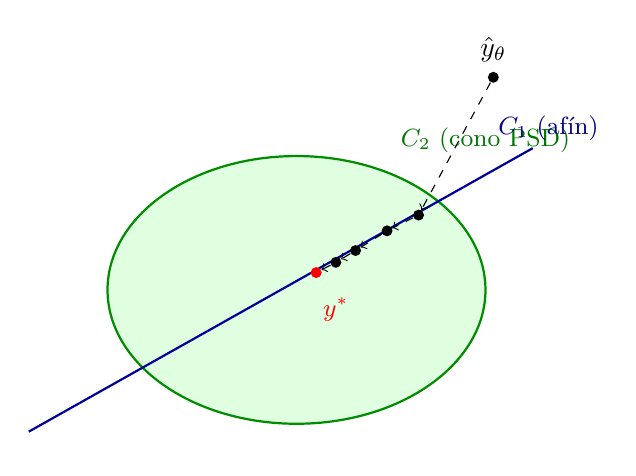
\begin{tikzpicture}[
        punto/.style={circle, fill=black, inner sep=1.4pt},
        etiqueta/.style={font=\small}
    ]
        % Cono PSD C2 (representación esquemática, no a escala)
        \begin{scope}
            \clip (-2.6,-2.2) rectangle (3.6,3.0);
            \fill[green!12] (0.2,-0.2) ellipse (2.4cm and 1.7cm);
        \end{scope}
        \draw[green!55!black, thick] (0.2,-0.2) ellipse (2.4cm and 1.7cm);
        \node[etiqueta, green!45!black] at (2.6,1.7) {$C_2$ (cono PSD)};

        % Subespacio afín C1 (recta)
        \draw[blue!60!black, thick] (-3.2,-2.0) -- (3.2,1.6);
        \node[etiqueta, blue!50!black] at (3.4,1.85) {$C_1$ (afín)};

        % Punto inicial
        \node[punto, label=above:{$\hat{y}_\theta$}] (start) at (2.7,2.5) {};

        % Trayectoria en zigzag
        \node[punto] (u1) at (1.75,0.75) {};
        \node[punto] (v1) at (1.35,0.55) {};
        \node[punto] (u2) at (0.95,0.30) {};
        \node[punto] (v2) at (0.70,0.15) {};
        \node[punto, fill=red] (opt) at (0.45,0.02) {};
        \node[etiqueta, red] at (0.7,-0.45) {$y^*$};

        \draw[dashed, ->] (start) -- (u1);
        \draw[dashed, ->] (u1) -- (v1);
        \draw[dashed, ->] (v1) -- (u2);
        \draw[dashed, ->] (u2) -- (v2);
        \draw[dashed, ->] (v2) -- (opt);
    \end{tikzpicture}%
    }
    \caption{Ilustración esquemática (no a escala) de la convergencia del algoritmo de 
    Douglas--Rachford: partiendo de una predicción $\hat{y}_\theta$ fuera de la región factible, 
    las proyecciones alternadas sobre el subespacio afín $C_1$ y el cono $C_2$ generan una 
    trayectoria en zigzag de amplitud decreciente que converge al punto factible 
    $y^*\in C_1\cap C_2$.}
    \label{fig:dr_geometrico}
\end{figure}






\subsection{Pase hacia Atrás: Cálculo del Gradiente a través de la Proyección}
\label{subsec:backward_pass}

Para que la red neuronal actualice sus pesos mediante retropropagación, es necesario calcular 
el gradiente de la función de pérdida con respecto a los parámetros del \textit{backbone}, lo 
cual exige propagar el gradiente a través de la capa de proyección iterativa. Al no ser esta 
una función explícita sino el resultado de un proceso de optimización de punto fijo, existen 
dos estrategias fundamentalmente distintas para calcular esta propagación, formalizadas de 
manera general en la Fase 2 del Algoritmo~\ref{algo:projection_layer} (Sección~\ref{sec:teorico}).

%\subsubsection{Desenrollado Algorítmico (Algorithm Unrolling)}

%La estrategia empleada en esta implementación trata cada iteración del ciclo de Douglas-Rachford 
%como una capa adicional, diferenciable, dentro del grafo computacional. Si el algoritmo se itera 
%$K$ veces, dicho ciclo se ``desenrolla'' en $K$ operaciones secuenciales, y el motor de 
%diferenciación automática de PyTorch aplica la regla de la cadena a través de todas ellas hasta 
%alcanzar los pesos del \textit{backbone}. Esta estrategia tiene la ventaja de ser directa de 
%implementar --- no requiere derivar analíticamente ninguna expresión adicional --- pero su costo 
%de memoria crece linealmente con el número de iteraciones $K$, ya que el grafo computacional 
%completo debe almacenarse para el cálculo posterior del gradiente.






\subsection{Pase hacia Atrás: Diferenciación Implícita}
\label{subsec:backward_pass}

Para entrenar la red es necesario propagar el gradiente de la pérdida a través de la 
capa de proyección. Dado que esta no es una función explícita sino el resultado de un 
proceso iterativo, la formulación original resuelve el problema mediante 
\textbf{diferenciación implícita}, siguiendo el esquema introducido en 
\cite{grontas2026pinet} y común a las arquitecturas de punto fijo diferenciables 
\cite{bai2019deq, gould2021ddn}. La observación central es que el estado de 
convergencia $s^* = (y^*, x^*)$ es, por definición, un punto fijo del operador $T$ de 
una iteración de Douglas--Rachford:
\begin{equation}
    s^* = T(s^*, \hat{y}_\theta).
    \label{eq:punto_fijo}
\end{equation}
Diferenciando ambos lados mediante el Teorema de la Función Implícita, el gradiente de 
la salida respecto de la predicción cruda satisface el sistema lineal
\begin{equation}
    \left(I - \frac{\partial T}{\partial s}\Big|_{s^*}\right) 
    \frac{\partial s^*}{\partial \hat{y}_\theta} 
    = \frac{\partial T}{\partial \hat{y}_\theta}\Big|_{s^*},
    \label{eq:diferenciacion_implicita}
\end{equation}
evaluado únicamente en el punto de convergencia, sin almacenar iteración intermedia 
alguna. En la práctica no se resuelve el sistema completo: durante la retropropagación 
solo se requiere el producto vector-Jacobiana (VJP) del gradiente entrante contra esta 
Jacobiana, lo que se obtiene resolviendo un único sistema lineal adjunto por muestra y 
aplicando diferenciación automática a una sola iteración del operador $T$ 
\cite{tang2026lminet, grontas2026pinet}.

Las consecuencias prácticas de este diseño son dos. Primero, el costo de memoria del 
pase hacia atrás es constante respecto del número de iteraciones del solucionador, lo 
que permite entrenar con un número elevado de iteraciones ($500$ en los experimentos 
del artículo) sin tener problemas de memoria. Segundo, el gradiente obtenido es el gradiente 
exacto en el punto fijo, y no una aproximación dependiente de la profundidad del 
desenrollado. Como se discutirá en la Sección~\ref{sec:extension_lpv}, esta exactitud 
interactúa de manera no trivial con la elección de la función de pérdida, hallazgo que 
motiva una de las contribuciones experimentales de esta memoria.





%\begin{table}[htpb]
%\centering
%\caption{Comparación entre desenrollado algorítmico y diferenciación implícita}
%\label{tab:comparacion_backward}
%\begin{tabular}{@{}p{3.2cm}p{5cm}p{5cm}@{}}
%\toprule
%\textbf{Criterio} & \textbf{Desenrollado} & \textbf{Diferenciación implícita} \\ \midrule
%Costo de memoria & $O(K)$, crece con las iteraciones & $O(1)$, independiente de $K$ \\
%Exactitud del gradiente & Aproximado si se trunca antes de converger & Exacto en el punto 
%fijo $s^*$ \\
%Acoplamiento profundidad-memoria & Sí: obliga a truncar el entrenamiento ($K\approx30$) & 
%No: permite converger profundamente también en entrenamiento \\
%Implementación & Diferenciación automática nativa sobre el bucle & Diferenciación automática 
%de una iteración + resolución de un sistema lineal por muestra \\ \bottomrule
%\end{tabular}
%\end{table}

\subsubsection{Interacción entre el Gradiente y el Criterio de Desempeño}

Ambas estrategias fueron implementadas sobre el mismo núcleo de proyección, de manera 
intercambiable con cualquier arquitectura de \textit{backbone}, lo que permitió compararlas 
empíricamente bajo condiciones idénticas (Capítulo~\ref{sec:experimentos}). Los resultados 
revelan una interacción no evidente entre la exactitud del gradiente y la función de pérdida 
empleada: dado que el criterio de desempeño alcanza su óptimo sobre la frontera del conjunto 
factible, el gradiente exacto de la diferenciación implícita ---o, equivalentemente, el de un 
desenrollado con un número elevado de iteraciones--- conduce a la red a proponer certificados 
próximos al borde de factibilidad, degradando la tasa de estabilización efectiva. El 
truncamiento del desenrollado a un número reducido de iteraciones introduce, en cambio, una 
imprecisión que opera como regularización implícita hacia certificados más conservadores.

En consecuencia, la elección del desenrollado truncado como estrategia por defecto en este 
trabajo no responde a una limitación de implementación, sino a una decisión informada por la 
evidencia experimental. Aprovechar plenamente las ventajas teóricas de la diferenciación 
implícita (gradiente exacto y memoria constante) requeriría reformular la función de pérdida 
para incorporar un margen explícito respecto de la frontera factible, extensión que se 
discute como línea de trabajo futuro en la Sección~\ref{sec:conclusiones}.








\subsection{Configuración de Entrenamiento de la Formulación Original}
\label{subsec:receta_paper}

El \textit{backbone} empleado en el artículo consiste de un Perceptrón 
Multicapa de dos capas ocultas de $64$ neuronas con activación ReLU, entrenado con 
Adam. Durante el entrenamiento, la capa de proyección ejecuta $500$ iteraciones de 
Douglas--Rachford con peso de anclaje $\sigma = 0.01$; en inferencia, el número de 
iteraciones se trata como un parámetro libre que intercambia velocidad por precisión 
de factibilidad sin necesidad de reentrenar.


\pendiente{incluir estos datos en una tabla mejor?}

La función de pérdida del artículo combina el criterio de desempeño con un término de 
regularización espectral:
\begin{equation}
    \mathcal{L}(\theta) = \frac{1}{N_{train}} \sum_{i=1}^{N_{train}} \Big[ 
    \log\det\big(Q^{(i)}\big) 
    \;-\; \beta_{soft}\, \lambda_{min}\big(F(y^{*(i)})\big) \Big], 
    \qquad \beta_{soft} = 100,
    \label{eq:loss_aumentada}
\end{equation}
evaluada sobre la salida proyectada $y^{*}$. El primer término minimiza el volumen del 
elipsoide invariante: dado que $\mathcal{E}(Q) = \{x : x^\top Q^{-1} x \le 1\}$ tiene 
volumen proporcional a $\sqrt{\det(Q)}$, minimizar $\log\det(Q)$ confina los estados en la región de atracción más compacta posible. \pendiente{agregar figura que muestre gráficamente lo que implica minimizar el elipsoide invariante} El 
segundo término cumple una doble función según el signo del autovalor mínimo de $F$: 
cuando es negativo, penaliza la violación residual de la restricción que subsiste tras 
un número finito de iteraciones del solucionador; cuando es positivo, recompensa que 
la solución mantenga un \textbf{margen} hacia el interior del cono, alejándola de la 
frontera de factibilidad. Este término de margen no es accesorio: contrarresta la 
tendencia natural del criterio de volumen, cuyo óptimo se sitúa exactamente sobre 
dicha frontera, y su rol resultará central en el análisis experimental de la 
Sección~\ref{sec:extension_lpv}.

Con esta configuración, el artículo reporta que la arquitectura alcanza cero 
violaciones de la restricción con $3000$--$4000$ iteraciones de inferencia, igualando 
la factibilidad del solucionador convexo de referencia (CVXPY/SCS) con tiempos de 
cómputo entre $3.5$ y $35$ veces menores, y manteniendo la estabilidad en lazo cerrado 
incluso sobre distribuciones de sistemas no vistas en entrenamiento.








\subsection{Limitaciones de la Formulación Original}
\label{subsec:limitaciones_vanilla}

La formulación original, si bien introduce un mecanismo novedoso con garantías 
formales de factibilidad, presenta limitaciones inherentes a su diseño y a su 
protocolo de validación. Identificarlas con precisión es relevante porque varias de 
ellas motivan directamente el aporte de esta memoria.

\subsubsection{Validación Restringida a Sistemas LTI Individuales de Baja Dimensión}
Los experimentos del artículo se limitan a sistemas de segundo orden ($n_x = 2$) con 
un actuador, donde cada instancia es un único sistema LTI. La arquitectura no fue 
evaluada sobre familias de sistemas que deban compartir un certificado común de 
estabilidad, escenario estructuralmente más exigente que constituye el núcleo del 
control robusto politópico. Adicionalmente, la parametrización de entrada 
$\operatorname{vech}(A)$ y la construcción espectral de los conjuntos de datos 
restringen los experimentos a matrices de estado simétricas, una clase de dinámicas de 
espectro real que excluye, entre otros, los modos oscilatorios y los fenómenos de 
crecimiento transitorio asociados a la no-normalidad.

\subsubsection{Rigidez Dimensional del \textit{Backbone}}
El \textit{backbone} asume una dimensionalidad de entrada fija, determinada por el 
tamaño del vector $\xi$. Los propios autores señalan como trabajo futuro la necesidad 
de escalar hacia \textit{``advanced backbone architectures''} para problemas de mayor 
dimensión. Esta limitación se agudiza en el contexto politópico, donde la descripción 
del sistema deja de ser un vector de tamaño fijo para convertirse en un conjunto de 
cardinalidad variable, como se desarrolla en la Sección~\ref{sec:extension_lpv}.

\subsubsection{Hiperparámetros de Margen Estáticos}
Tanto el margen de positividad $\epsilon$ como el multiplicador $\alpha_s$ se fijan a 
priori como constantes globales, sin mecanismo para adaptarlos a la dificultad de cada 
instancia. Para sistemas próximos al borde de la estabilizabilidad, la región factible 
resultante puede ser geométricamente delgada, ralentizando la convergencia del 
solucionador iterativo.

\subsubsection{Supuesto de Factibilidad A Priori}
La arquitectura no contempla el caso en que la instancia recibida sea infactible 
($C_1 \cap C_2 = \emptyset$): la garantía de convergencia del Teorema de 
Douglas--Rachford presupone intersección no vacía. El propio protocolo experimental 
del artículo lo evidencia, al filtrar explícitamente de sus conjuntos de datos las 
muestras cuyo par $(A, B)$ no es estabilizable. En esta memoria, dicho supuesto se 
satisface por construcción al emplear una base de datos de sistemas certificadamente 
estabilizables (Sección~\ref{sec:base_datos}).




\section{Extensión a la Estabilización Robusta de Sistemas Politópicos}
\label{sec:extension_lpv}

La formulación original de LMI-Net, descrita en la 
Sección~\ref{sec:arquitectura_lminet}, fue propuesta y validada para instancias LTI 
individuales. Esta sección desarrolla el aporte central de esta memoria: la extensión 
de dicha arquitectura a la estabilización robusta de sistemas LPV politópicos, una 
clase de problemas estructuralmente más exigente que no fue evaluada en el trabajo 
original. La extensión se articula en torno a dos ejes de diseño ortogonales entre sí, 
que en conjunto definen el espacio experimental de esta investigación: el primero 
concierne a la representación y procesamiento de la entrada cómo una red 
neuronal debe ingerir un polítopo de cardinalidad variable---, y se desarrolla en la 
Sección~\ref{sec:arquitecturas}; el segundo concierne a la \textbf{estrategia de 
retropropagación} a través de la capa de proyección, donde esta memoria introduce y 
estudia una alternativa al esquema implícito original.

\subsection{El Problema: Estabilizabilidad Cuadrática con Tasa de Decaimiento}
\label{subsec:problema_politopico}

Considérese el sistema politópico presentado en el Marco Teórico 
(Sección~\ref{sec:teorico}), definido por la envolvente convexa de $N$ vértices:
\begin{equation}
    \dot{x} = A(\theta)x + B(\theta)u, \qquad 
    \big(A(\theta), B(\theta)\big) = \sum_{i=1}^{N} \theta_i (A_i, B_i), \qquad 
    \theta \in \Delta_N,
    \label{eq:sistema_politopico}
\end{equation}
donde $\Delta_N$ denota el símplex unitario. Se busca una única ley de realimentación 
estática $u = Kx$, común a todo el polítopo, que garantice estabilidad exponencial con 
tasa de decaimiento prescrita $\alpha > 0$ para toda trayectoria admisible del 
parámetro. Bajo la parametrización $Q = P^{-1}$, $Y = KQ$, dicha garantía se obtiene 
si el par $(Q, Y)$ satisface simultáneamente las $N+1$ condiciones
\begin{equation}
    A_i Q + Q A_i^\top + B_i Y + Y^\top B_i^\top + 2\alpha Q \prec 0 
    \quad \forall i \in \{1, \dots, N\}, 
    \qquad Q \succeq \epsilon I.
    \label{eq:lmis_vertices}
\end{equation}
La suficiencia de verificar únicamente los vértices se sigue de la afinidad de la 
expresión de Lyapunov en el par $(A, B)$: para cualquier $\theta \in \Delta_N$, el 
lado izquierdo evaluado en $\big(A(\theta), B(\theta)\big)$ es exactamente la 
combinación convexa, con pesos $\theta_i$, de los lados izquierdos evaluados en cada 
vértice; una combinación convexa de matrices definidas negativas es definida negativa 
\cite{boyd1994lmi}. Más aún, dado que el certificado $V(x) = x^\top Q^{-1} x$ es 
independiente del parámetro, la garantía de decaimiento se sostiene para variaciones 
arbitrariamente rápidas de $\theta(t)$, propiedad conocida como estabilidad 
cuadrática. Esta robustez tiene como contraparte un grado de conservadurismo: exigir 
un certificado común a todos los vértices es una condición suficiente pero no 
necesaria para la estabilizabilidad del polítopo.






\subsection{Construcción Bloque-Diagonal: de $N+1$ Desigualdades a Una}
\label{subsec:construccion_bloques}

La formulación general del problema parametrizado 
(Ec.~\eqref{eq:problema_parametrizado}) admite, como observan los propios autores, la 
representación de múltiples LMIs simultáneas mediante una única matriz bloque-diagonal 
\cite{tang2026lminet}. Sin embargo, el trabajo original no instancia ni evalúa esta 
posibilidad: sus experimentos involucran una única desigualdad por sistema. El aporte 
metodológico de esta memoria consiste en explotar dicha estructura para el caso 
robusto politópico, apilando las $N$ condiciones de vértice y la condición de 
positividad de la Ec.~\eqref{eq:lmis_vertices} en un único mapa afín:
\begin{equation}
    F(y) = \operatorname{diag}\Big( 
        F^{(1)}(y),\; \dots,\; F^{(N)}(y),\; Q - \epsilon I 
    \Big) \succeq 0,
    \label{eq:F_politopica}
\end{equation}
donde cada bloque de vértice se define como
\begin{equation}
    F^{(i)}(y) = -\big( A_i Q + Q A_i^\top + B_i Y + Y^\top B_i^\top + 2\alpha Q \big).
    \label{eq:bloque_vertice_lpv}
\end{equation}
Dado que una matriz bloque-diagonal es semidefinida positiva si y solo si todos sus 
bloques lo son, la condición $F(y) \succeq 0$ es exactamente equivalente al sistema de 
la Ec.~\eqref{eq:lmis_vertices}. La consecuencia central de esta construcción es que 
\textbf{la maquinaria de proyección descrita en la 
Sección~\ref{sec:arquitectura_lminet} se preserva íntegra}: $F$ sigue siendo afín en 
$y$, por lo que el subespacio $C_1$, la matriz precomputada 
$M^{-1} = (I + L^\top L)^{-1}$ y el Algoritmo~\ref{algo:dr_concreto} operan sin 
modificación alguna; lo único que cambia es la dimensión del espacio levantado, cuyo 
número de bloques pasa de $2$ a $N+1$.

La estructura bloque-diagonal no es únicamente una conveniencia notacional. La proyección sobre el cono PSD se realiza bloque a bloque, 
mediante $N+1$ descomposiciones espectrales independientes de matrices $n_x \times 
n_x$, con costo $O\big((N+1)\, n_x^3\big)$; tratar $F$ como una matriz monolítica de 
dimensión $(N+1)n_x$ elevaría dicho costo a $O\big((N+1)^3 n_x^3\big)$. 
Adicionalmente, la matriz $M^{-1}$ de la proyección afín conserva la dimensión del 
vector de decisión ($\dim y \times \dim y$), independiente de $N$: el crecimiento del 
polítopo engrosa el operador $L$, pero no el sistema lineal que se resuelve en cada 
iteración. Estas propiedades anticipan un comportamiento de escalamiento favorable 
frente a solucionadores genéricos, hipótesis que se evalúa empíricamente en el 
Capítulo~\ref{sec:experimentos}.











\subsection{Adaptación del Problema de Referencia}
\label{subsec:adaptacion_db}

La instancia experimental de esta memoria difiere de la del artículo original en un 
aspecto impuesto por los datos disponibles: la base UNICAMP 
(Sección~\ref{sec:base_datos}) caracteriza cada sistema únicamente por sus vértices 
$\{(A_i, B_i)\}$, sin incluir el canal de perturbación exógena $B_w$. En consecuencia, 
el problema de diseño conjunto bajo perturbación acotada de la 
Ec.~\eqref{eq:lmi_conjunta_lti} no es reproducible sobre esta base, y el criterio de 
certificación adoptado es la estabilización robusta con tasa de decaimiento prescrita 
de la Ec.~\eqref{eq:lmis_vertices}, con $\alpha = 0.01$ fijo en los experimentos 
principales. Cabe precisar que el elipsoide $\mathcal{E}(Q) = \{x : x^\top Q^{-1} x 
\le 1\}$ conserva su carácter de conjunto invariante ---como conjunto de nivel del 
certificado de Lyapunov del lazo cerrado---, aunque su interpretación deja de estar 
ligada al rechazo de una perturbación específica. La Tabla~\ref{tab:migracion} resume 
la correspondencia completa entre ambas instancias.

\begin{table}[htpb]
\centering
\caption{Correspondencia entre la instancia original de LMI-Net y la extensión 
politópica de esta memoria}
\label{tab:migracion}
\begin{tabular}{@{}p{3.6cm}p{4.8cm}p{4.8cm}@{}}
\toprule
 & \textbf{Original \cite{tang2026lminet}} & \textbf{Esta memoria} \\ \midrule
Clase de sistema & LTI individual con perturbación & LPV politópico, $N$ vértices \\
Parámetro de entrada $\xi$ & $(A, B, B_w)$, dimensión fija & $\{(A_i, B_i)\}_{i=1}^N$, 
cardinalidad variable \\
Escalar en la LMI & $\alpha_s$: multiplicador del procedimiento S & $\alpha$: tasa de 
decaimiento prescrita \\
Bloques de $F(y)$ & $2$ (desigualdad conjunta; positividad) & $N+1$ ($N$ vértices; 
positividad) \\
Garantía certificada & Invarianza de $\mathcal{E}(Q)$ bajo $w^\top w \le 1$ & Decaimiento 
exponencial robusto a tasa $\alpha$ \\
Capa de proyección & \multicolumn{2}{c}{Idéntica (Algoritmo~\ref{algo:dr_concreto})} \\ 
\bottomrule
\end{tabular}
\end{table}














\subsection{Estrategia de Retropropagación Alternativa: Desenrollado Algorítmico}
\label{subsec:unrolling}

La formulación original calcula los gradientes exclusivamente mediante diferenciación 
implícita (Sección~\ref{subsec:backward_pass}). Esta memoria implementa adicionalmente 
una segunda estrategia, el \textbf{desenrollado algorítmico} (\textit{algorithm 
unrolling}), y estudia ambas de forma comparada. Su principio es directo: cada 
iteración del ciclo de Douglas--Rachford se trata como una capa diferenciable más del 
grafo computacional; si el solucionador ejecuta $K$ iteraciones, el motor de 
diferenciación automática aplica la regla de la cadena a través de las $K$ operaciones 
hasta alcanzar los pesos del \textit{backbone}. La estrategia no requiere derivación 
adicional alguna, pero su costo de memoria crece linealmente con $K$, pues el grafo 
completo debe almacenarse para el pase hacia atrás. Esto obliga, en la práctica, a 
truncar el número de iteraciones durante el entrenamiento muy por debajo del utilizado en inferencia, donde el pase hacia 
adelante no acarrea grafo y puede ejecutarse hasta la convergencia. Ambas estrategias 
comparten exactamente el mismo pase hacia adelante y son intercambiables con cualquier 
arquitectura de \textit{backbone}, lo que permite aislar experimentalmente el efecto 
del gradiente. La Tabla~\ref{tab:comparacion_backward} resume sus diferencias.

\begin{table}[htpb]
\centering
\caption{Comparación entre las dos estrategias de retropropagación}
\label{tab:comparacion_backward}
\begin{tabular}{@{}p{3.2cm}p{5cm}p{5cm}@{}}
\toprule
\textbf{Criterio} & \textbf{Diferenciación implícita} & \textbf{Desenrollado} \\ \midrule
Costo de memoria & $O(1)$, independiente de $K$ & $O(K)$, crece con las iteraciones \\
Gradiente & Exacto en el punto fijo & Aproximado si se trunca antes de converger \\
Profundidad en entrenamiento & Permite converger profundamente ($K = 500$) & Obliga a 
truncar ($K \approx 30$) \\
Implementación & Sistema lineal adjunto por muestra & Diferenciación automática nativa 
sobre el bucle \\ \bottomrule
\end{tabular}
\end{table}

A priori, la comparación parece favorecer sin ambigüedad a la diferenciación 
implícita: gradiente exacto y memoria constante. Sin embargo, esta memoria plantea 
como hipótesis de diseño ---y verifica experimentalmente en el 
Capítulo~\ref{sec:experimentos}--- que la exactitud del gradiente interactúa de manera 
no trivial con la función de pérdida: cuando el criterio de desempeño alcanza su 
óptimo sobre la frontera del conjunto factible, el gradiente exacto conduce a la red a 
proponer certificados al borde de la factibilidad, mientras que la imprecisión del 
desenrollado truncado opera como una regularización implícita hacia soluciones más 
conservadoras. Este fenómeno, no reportado en el trabajo original, ofrece además una 
explicación mecanística de una decisión de diseño que dicho trabajo emplea sin 
justificar: la inclusión del término de margen espectral en su función de pérdida, 
como se desarrolla a continuación.











\subsection{Funciones de Pérdida}
\label{subsec:perdidas}

Dado que la capa de proyección asume íntegramente la responsabilidad de la 
factibilidad, la función de pérdida cumple un rol distinto al habitual: no discrimina 
entre soluciones válidas e inválidas, sino que selecciona \emph{en qué punto de la 
región factible} se sitúa la solución. Esta memoria estudia una familia de tres 
funciones de pérdida que difieren precisamente en su tratamiento de la frontera de 
dicha región, todas evaluadas sobre la salida proyectada $(Q, Y)$.

\subsubsection{Pérdida de Referencia: Volumen con Margen Lineal}
La línea base es la pérdida de la formulación original 
(Ec.~\eqref{eq:loss_aumentada}): el criterio de volumen $\log\det(Q)$ aumentado con el 
término de margen espectral $-\beta_{soft}\,\lambda_{min}(F(y^*))$, con $\beta_{soft} 
= 100$, donde $\lambda_{min}$ del bloque-diagonal se calcula como el mínimo sobre los 
$N+1$ bloques de la Ec.~\eqref{eq:F_politopica}. El término de margen recompensa 
linealmente y sin cota el alejamiento de la frontera de factibilidad.

\subsubsection{Ablación: Volumen sin Margen}
La segunda variante elimina el término de margen, dejando únicamente 
$\mathcal{L} = \log\det(Q)$. Su propósito es diagnóstico: el óptimo de un criterio de 
volumen sin contrapeso se sitúa exactamente sobre la frontera del conjunto factible 
---donde las restricciones se activan---, por lo que esta ablación permite aislar y 
cuantificar el fenómeno de degradación por proximidad al borde descrito en la 
Sección~\ref{subsec:unrolling}, y con ello el rol real que el término de margen cumple 
en la receta original.

\subsubsection{Variante Propuesta: Margen con Umbral (\textit{Hinge})}
El margen lineal de la formulación original presenta un inconveniente conceptual: 
recompensa el alejamiento de la frontera de forma ilimitada, compitiendo contra el 
criterio de desempeño incluso cuando la solución ya dispone de un margen holgado. Esta 
memoria propone como variante una penalización con umbral prescrito $m > 0$:
\begin{equation}
    \mathcal{L}_{hinge} = \log\det(Q) + \beta \cdot 
    \operatorname{relu}\big(m - \lambda_{min}(F(y^*))\big)^2,
    \label{eq:loss_hinge}
\end{equation}
que penaliza cuadráticamente la insuficiencia de margen por debajo de $m$ y se anula 
por completo sobre dicho umbral, permitiendo que el criterio de volumen opere sin 
interferencia una vez asegurada una distancia mínima a la frontera. Esta construcción 
formaliza la noción de \emph{margen prescrito} que el análisis experimental identifica 
como condición para aprovechar el gradiente exacto de la diferenciación implícita.










\subsection{El Problema de la Representación: el Polítopo como Conjunto}
\label{subsec:politopo_conjunto}

Queda por resolver la interfaz entre el sistema politópico y el \textit{backbone}. La 
adaptación directa de la arquitectura original consiste en aplanar y concatenar todos 
los vértices en un único vector de características, de dimensión $N(n_x^2 + n_x n_u)$ 
---por ejemplo, $24$ entradas para la configuración $n_x = 3$, $n_u = 1$, $N = 2$, con 
salida de $\dim y = \frac{n_x(n_x+1)}{2} + n_u n_x = 9$ parámetros. Esta 
representación, empleada como línea base en esta memoria, arrastra dos defectos 
estructurales. El primero es la \textbf{rigidez de cardinalidad}: la dimensión de 
entrada depende de $N$, obligando a entrenar una arquitectura distinta para cada 
tamaño de polítopo. El segundo es más sutil: un polítopo es matemáticamente un 
\textbf{conjunto} de vértices, sin orden intrínseco ---permutar los vértices describe 
exactamente el mismo sistema incierto y admite exactamente el mismo certificado---, 
pero el vector aplanado impone un orden arbitrario, forzando a la red a consumir 
capacidad y datos en aprender una invarianza que la estructura del problema otorga de 
antemano. La resolución de ambos defectos mediante sesgos inductivos de conjunto 
constituye el primer eje de diseño de esta memoria y se desarrolla en la sección 
siguiente.













% =====================================================================
%  Análisis de la base de datos de control robusto (DB_ssf_RS_500_c.mat)
%  Sección lista para % =====================================================================
%  Análisis de la base de datos de control robusto (DB_ssf_RS_500_c.mat)
%  Sección lista para % =====================================================================
%  Análisis de la base de datos de control robusto (DB_ssf_RS_500_c.mat)
%  Sección lista para % =====================================================================
%  Análisis de la base de datos de control robusto (DB_ssf_RS_500_c.mat)
%  Sección lista para \input{analisis_db.tex}
%  Requiere: graphicx, booktabs, amsmath, amssymb
%  \graphicspath{{figuras/}}  % o ajusta la ruta a tus figuras
% =====================================================================

\section{Caracterización de la base de datos}
\label{sec:analisis-db}

% --------------------------------------------------------------------
\subsection{Propósito y estructura}
% --------------------------------------------------------------------

La base de datos \texttt{DB\_ssf\_RS\_500\_c.mat} es el conjunto de
entrenamiento del modelo. Cada muestra describe un \emph{sistema dinámico
incierto} junto con un controlador que lo estabiliza. Conviene fijar primero la
intuición de qué es cada cosa antes de cuantificarla.

Un \textbf{sistema lineal} modela cómo evoluciona en el tiempo un vector de
estado $x(t)\in\mathbb{R}^{n_x}$ (las variables internas del proceso) cuando se
le aplica una señal de control $u(t)\in\mathbb{R}^{n_u}$:
%
\begin{equation}
  \dot{x}(t) = A\,x(t) + B\,u(t).
  \label{eq:lti}
\end{equation}
%
La matriz $A$ codifica la \emph{dinámica propia} del sistema (cómo se influyen
entre sí las variables si no hiciéramos nada), y $B$ describe \emph{cómo entra
el control} en esa dinámica. El número $n_x$ es el \emph{orden} (cuántas
variables de estado) y $n_u$ es el número de \emph{actuadores} (cuántas
perillas de control independientes hay).

En la práctica el sistema no se conoce con exactitud: hay incertidumbre en sus
parámetros. Se modela esa incertidumbre con un \textbf{politopo}, es decir, una
familia de sistemas posibles obtenida ``mezclando'' $N$ casos extremos
conocidos —los \emph{vértices} $(A_i,B_i)$— en todas las proporciones
convexas:
%
\begin{equation}
  \bigl(A(\theta),B(\theta)\bigr)=\sum_{i=1}^{N}\theta_i\,(A_i,B_i),
  \qquad \theta_i\ge 0,\ \textstyle\sum_i\theta_i=1.
  \label{eq:politopo}
\end{equation}
%
Intuitivamente, el sistema real es \emph{algún} punto dentro de la envolvente
convexa de esos $N$ vértices, pero no sabemos cuál; un controlador
\emph{robusto} debe funcionar para todos a la vez. Esto es análogo, en
términos de computación, a exigir una garantía en el \emph{peor caso} sobre un
conjunto acotado de entradas posibles.

Cada muestra de la base es por tanto una terna: el conjunto de vértices
$\{A_i\}$, el conjunto $\{B_i\}$, y una \textbf{ganancia} $K\in\mathbb{R}^{n_u\times
n_x}$ que define el controlador por realimentación de estado $u(t)=K\,x(t)$ —una
única $K$ que estabiliza todo el politopo (Tabla~\ref{tab:esquema}). La etiqueta
\texttt{RS} (\emph{robustly stabilizable}) indica que el sistema admite tal
ganancia robusta.\footnote{\textbf{Procedencia (por confirmar con el autor de la
base):} la evidencia empírica (Sec.~\ref{sec:db-control}) es consistente con que
cada $K$ se obtuvo resolviendo un problema de factibilidad (una LMI de
estabilizabilidad cuadrática), sin optimizar la rapidez de la respuesta. Falta
confirmar cómo se generaron los vértices $(A_i,B_i)$.}

\begin{table}[t]
  \centering
  \caption{Esquema de la base de datos. Cada sistema es un politopo de $N$
  vértices con una ganancia robusta $K$.}
  \label{tab:esquema}
  \begin{tabular}{llll}
    \toprule
    Campo & Símbolo & Forma & Descripción \\
    \midrule
    \texttt{A} & $\{A_i\}_{i=1}^N$ & $N\times(n_x\!\times\! n_x)$ & Dinámica propia de cada vértice \\
    \texttt{B} & $\{B_i\}_{i=1}^N$ & $N\times(n_x\!\times\! n_u)$ & Entrada de control de cada vértice \\
    \texttt{K} & $K$               & $n_u\times n_x$             & Ganancia del controlador (común) \\
    \midrule
    \multicolumn{4}{l}{$n_x\in\{2,3,4,5\}$\quad $n_u\in\{1,2\}$\quad $N\in\{2,3,4,5\}$\quad $500$ casos/celda} \\
    \bottomrule
  \end{tabular}
\end{table}

% --------------------------------------------------------------------
\subsection{Cómo se mide un sistema y su estabilidad}
\label{sec:db-conceptos}
% --------------------------------------------------------------------

Para caracterizar la base usamos un puñado de indicadores numéricos. Como el
lector no tiene por qué venir de teoría de control, los explicamos aquí en
lenguaje llano; la Tabla~\ref{tab:glosario} los resume.

\paragraph{Estabilidad y autovalores.}
La pregunta central sobre un sistema es si es \emph{estable}: si lo perturbamos,
¿vuelve al equilibrio o se dispara? Para un sistema lineal
$\dot{x}=Ax$, la respuesta la dan los \textbf{autovalores} de $A$. Toda
solución es una combinación de ``modos'' de la forma $e^{\lambda t}$, donde
$\lambda=a+bi$ es un autovalor. Su \emph{parte real} $a=\operatorname{Re}\lambda$
controla la magnitud ($e^{at}$ crece si $a>0$ y decae si $a<0$) y su parte
imaginaria $b$ controla la oscilación. Por tanto:
%
\begin{center}
  \emph{el sistema es estable} $\iff$ \emph{todos} sus autovalores cumplen
  $\operatorname{Re}\lambda<0$.
\end{center}
%
En el plano complejo, esto es ``todos los autovalores en el semiplano
izquierdo''.

\paragraph{Abscisa espectral: el modo que decide.}
No hace falta mirar todos los autovalores: basta el \emph{peor}. La
\textbf{abscisa espectral} es el mayor de las partes reales,
$\max\operatorname{Re}\lambda(A)$. Es el modo que crece más rápido (o decae más
lento) y, por sí solo, decide la estabilidad: si la abscisa es negativa, todos
los modos decaen; si es positiva, al menos uno explota. Un valor de, por
ejemplo, $832$ significa que el modo dominante crece como $e^{832\,t}$: una
inestabilidad extremadamente violenta. Lo usamos como \emph{medida relativa de
qué tan inestable} es una planta (no tiene unidades físicas porque los sistemas
son sintéticos).

\paragraph{Los dos ``máximos''.}
En las fórmulas aparecen \emph{dos} máximos anidados, y conviene separarlos:
%
\begin{equation*}
  \underbrace{\max_{i=1,\dots,N}}_{\text{(2) peor \emph{vértice}}}
  \ \underbrace{\max\,\operatorname{Re}\,\lambda(A_i)}_{\text{(1) peor \emph{modo} de ese vértice}}.
\end{equation*}
%
El máximo interno (1) recorre los autovalores de \emph{un} vértice y se queda
con su modo dominante (la abscisa espectral de $A_i$). El máximo externo (2)
recorre los $N$ vértices del politopo y se queda con el más desfavorable. La
combinación es la lectura de \emph{peor caso}: ``de toda la familia de sistemas
posibles, ¿qué tan mal se comporta el peor de ellos?''.

\paragraph{Norma de una matriz: su ``tamaño''.}
La norma espectral $\lVert A\rVert_2$ mide cuánto puede \emph{amplificar} esa
matriz a un vector (formalmente, su mayor valor singular). Es una medida del
``tamaño'' o la fuerza de la dinámica: una $\lVert A\rVert_2$ grande indica
acoplamientos internos intensos. Reportamos $\max_i\lVert A_i\rVert_2$, el
tamaño del vértice más grande del politopo.

\paragraph{Tasa de decaimiento $\alpha$: el margen de seguridad.}
Una vez cerrado el lazo con el controlador, la matriz que gobierna la dinámica
pasa a ser $A_i+B_iK$. Su abscisa espectral, cambiada de signo, es la
\textbf{tasa de decaimiento}
$\alpha=-\max_i\max\operatorname{Re}\lambda(A_i+B_iK)$. Mide \emph{qué tan
rápido} se extingue la peor respuesta: $\alpha>0$ garantiza estabilidad, y
cuanto mayor sea $\alpha$, más rápido y con más margen vuelve el sistema al
equilibrio. Un $\alpha\approx0$ significa ``estable, pero al borde'': el sistema
apenas se sostiene sobre la frontera de la inestabilidad.

\paragraph{Otros indicadores.}
La \emph{dispersión del politopo} $\max_i\lVert A_i-\bar A\rVert_2$ (con $\bar A$
el promedio de los vértices) mide qué tan distintos son los vértices entre sí,
es decir, cuánta incertidumbre hay. El \emph{número de condición} $\kappa(A_i)$
mide la sensibilidad numérica de la matriz (valores altos anticipan problemas de
precisión). El \emph{esfuerzo de control} $\lVert K\rVert_2$ mide qué tan
``agresivo'' es el controlador.

\begin{table}[t]
  \centering
  \caption{Glosario de indicadores usados en el análisis.}
  \label{tab:glosario}
  \small
  \begin{tabular}{p{3.0cm}p{3.4cm}p{6.6cm}}
    \toprule
    Indicador & En palabras simples & Un valor alto significa\dots \\
    \midrule
    Abscisa espectral (lazo abierto)\newline $\max_i\max\operatorname{Re}\lambda(A_i)$
      & Rapidez del modo más inestable del peor vértice
      & Planta muy inestable: sin control, se dispara muy rápido. \\
    Tasa de decaimiento\newline $\alpha=-\max_i\max\operatorname{Re}\lambda(A_i+B_iK)$
      & Qué tan rápido se calma el sistema ya controlado
      & Más margen de estabilidad; $\alpha\approx0$ = estable al borde. \\
    Norma $\max_i\lVert A_i\rVert_2$
      & ``Tamaño''/fuerza de la dinámica propia
      & Acoplamientos internos intensos. \\
    Norma $\max_i\lVert B_i\rVert_2$
      & Cuánto influye el control en el estado
      & Actuadores con mucha autoridad. \\
    Dispersión del politopo\newline $\max_i\lVert A_i-\bar A\rVert_2$
      & Qué tan distintos son los vértices
      & Más incertidumbre que cubrir con una sola $K$. \\
    Condición $\kappa(A_i)$
      & Sensibilidad numérica de la matriz
      & Riesgo de imprecisión numérica. \\
    Esfuerzo $\lVert K\rVert_2$
      & Qué tan ``fuerte'' es el controlador
      & Acción de control más agresiva. \\
    \bottomrule
  \end{tabular}
\end{table}

% --------------------------------------------------------------------
\subsection{Cobertura y diseño experimental}
% --------------------------------------------------------------------

El archivo organiza las muestras en un arreglo de cuatro índices,
$\texttt{BASE}[\,n_x,\,n_u,\,N,\,\text{caso}\,]$, de forma nominal
$5\times 2\times 5\times 500$. La malla está poblada parcialmente: el orden
mínimo depende del número de actuadores ($n_u{=}1\Rightarrow n_x\in\{2,\dots,5\}$;
$n_u{=}2\Rightarrow n_x\in\{3,4,5\}$) y siempre $N\ge 2$. De las $25\,000$
posiciones nominales sólo $28$ están ocupadas, con exactamente $500$ casos cada
una: en total $\mathbf{14\,000}$ sistemas ($8\,000$ con $n_u{=}1$ y $6\,000$ con
$n_u{=}2$).

La base sigue así un \emph{diseño factorial completo y perfectamente
balanceado} sobre los factores $(n_x, n_u, N)$ admisibles
(Fig.~\ref{fig:cobertura}): las $28$ combinaciones válidas aparecen con la misma
cantidad de ejemplos ($500$), sin celdas faltantes ni sobre-representadas. Este
balance es deseable para el aprendizaje: evita que el modelo privilegie una
configuración por mero desbalance de frecuencia, y permite reportar métricas
separadas por $N$ y por $n_x$ sin correcciones.

\begin{figure}[t]
  \centering
  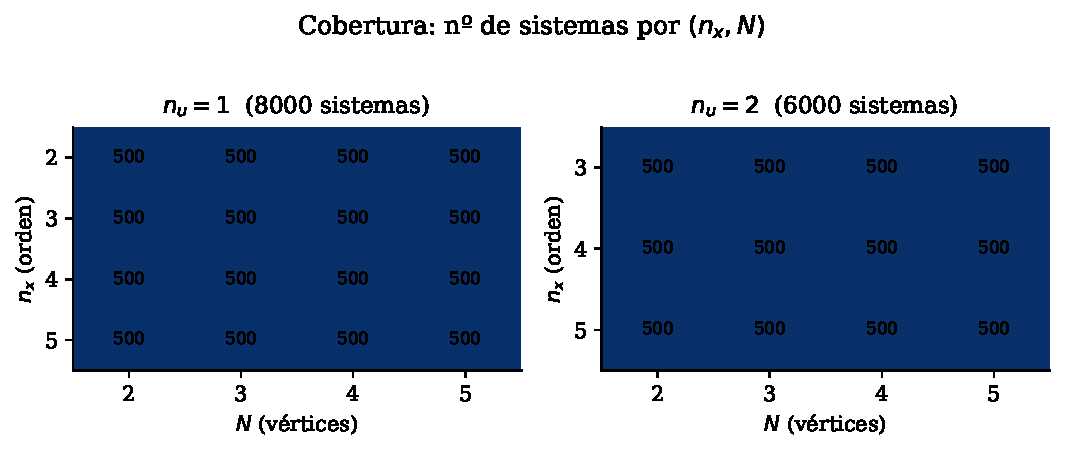
\includegraphics[width=\linewidth]{fig1_cobertura.pdf}
  \caption{Cobertura factorial: número de sistemas por $(n_x,N)$, separado por
  número de actuadores $n_u$. El soporte está completamente balanceado a $500$
  sistemas por celda.}
  \label{fig:cobertura}
\end{figure}

% --------------------------------------------------------------------
\subsection{La planta sin control (lazo abierto)}
\label{sec:db-ol}
% --------------------------------------------------------------------

``Lazo abierto'' se refiere al sistema \emph{sin} controlador. Las plantas de la
base son \emph{difíciles}: el $\mathbf{98.8\%}$ es inestable en lazo abierto
(al menos un vértice tiene un autovalor con parte real positiva), y sólo el
$1.2\%$ sería estable por sí solo. La abscisa espectral del peor vértice
(la rapidez del modo más inestable, ver Sec.~\ref{sec:db-conceptos}) tiene
mediana $30.9$ y llega hasta $\sim\!832$ (Fig.~\ref{fig:estabilidad}). En otras
palabras, la base no contiene casos triviales: el controlador debe
\emph{crear} la estabilidad, no sólo conservarla.

\begin{figure}[t]
  \centering
  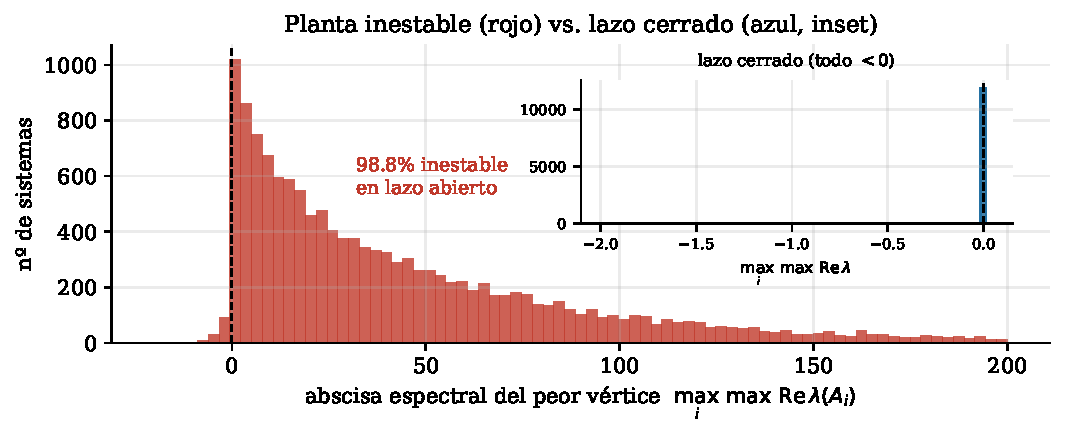
\includegraphics[width=\linewidth]{fig2_estabilidad.pdf}
  \caption{Abscisa espectral del peor vértice. Sin control la planta es
  inestable (rojo, parte real $>0$) en el $98.8\%$ de los casos; con la ganancia
  $K$ el lazo cerrado es estable en el $100\%$ (inset azul, todos $<0$).}
  \label{fig:estabilidad}
\end{figure}

En cuanto al ``tamaño'' de la dinámica (Fig.~\ref{fig:normas}), los descriptores
tienen un rango muy amplio: $\max_i\lVert A_i\rVert_2$ va de $12$ a $1012$
(mediana $131$) y crece de forma marcada con el orden $n_x$, mientras que
$\max_i\lVert B_i\rVert_2$ se mantiene acotado en $[0.74,\,16.8]$. Esta
disparidad de escalas —tres órdenes de magnitud en $\lVert A\rVert$— es
justamente la que obliga a \emph{normalizar} los datos antes de entrenar: cada
politopo se reescala dividiéndolo por su entrada de mayor magnitud,
$\gamma=\max(\max|A|,\max|B|)$, de modo que todas las cifras queden en
$[-1,1]$ y los sistemas sean comparables entre sí (esta reescala no cambia el
signo de los autovalores —y por tanto no afecta la estabilidad— aunque sí divide
la tasa de decaimiento por $\gamma$).

\begin{figure}[t]
  \centering
  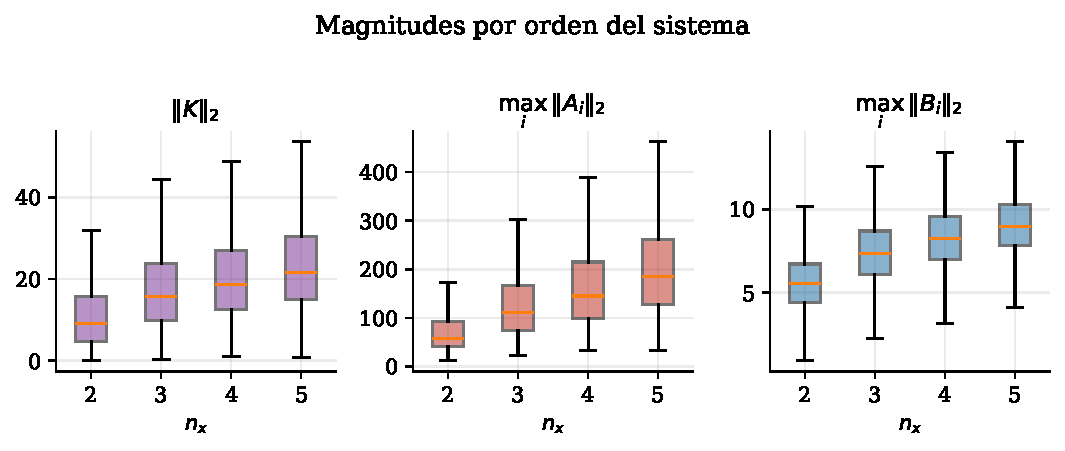
\includegraphics[width=\linewidth]{fig5_normas.pdf}
  \caption{Distribución del esfuerzo de control $\lVert K\rVert_2$ y de los
  tamaños $\max_i\lVert A_i\rVert_2$ y $\max_i\lVert B_i\rVert_2$, según el orden
  $n_x$. Ambos crecen con el orden del sistema.}
  \label{fig:normas}
\end{figure}

\paragraph{¿Se puede controlar? Controlabilidad y condicionamiento.}
Un requisito previo para que exista una ganancia estabilizante es que el sistema
sea \emph{controlable}: que desde la entrada se pueda influir en todas las
direcciones del estado. Esto se cumple en el $100\%$ de los vértices de todos
los sistemas. El número de condición de las matrices es benigno en general
($\kappa(A_i)$ con mediana $53$), con una cola pesada: un $0.39\%$ de los
sistemas supera $\kappa>10^4$, con casos extremos de hasta $5.7\times10^5$
(Fig.~\ref{fig:cond}); estos son los sistemas numéricamente delicados durante el
entrenamiento.

\begin{figure}[t]
  \centering
  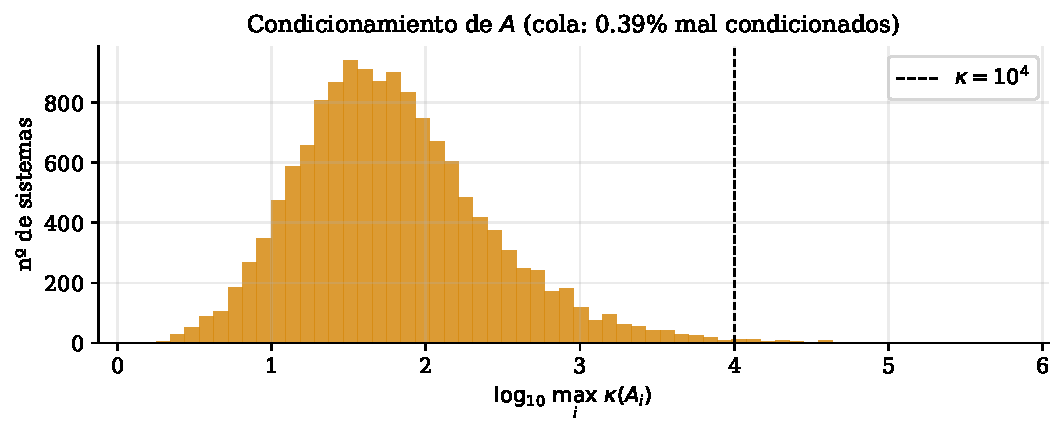
\includegraphics[width=0.82\linewidth]{fig7_condicionamiento.pdf}
  \caption{Número de condición $\max_i\kappa(A_i)$ (escala $\log_{10}$). La gran
  mayoría está bien condicionada; una cola del $0.39\%$ supera $\kappa=10^4$.}
  \label{fig:cond}
\end{figure}

% --------------------------------------------------------------------
\subsection{Tamaño de la incertidumbre (geometría del politopo)}
% --------------------------------------------------------------------

¿Qué tan ``grande'' es la incertidumbre de cada sistema? Lo medimos con la
dispersión de los vértices respecto a su promedio,
$\max_i\lVert A_i-\bar A\rVert_2$: si los vértices son muy parecidos entre sí, el
politopo es pequeño (poca incertidumbre); si son muy distintos, es grande. Su
mediana es $97.5$ y crece de forma sistemática con el número de vértices $N$
(Fig.~\ref{fig:dispersion}): más vértices implican politopos más amplios y, por
tanto, una incertidumbre más severa que la \emph{misma} ganancia $K$ debe cubrir
a la vez. Esto convierte a $N$ en un eje natural de dificultad y motiva evaluar
el modelo \emph{separado por $N$}.

\begin{figure}[t]
  \centering
  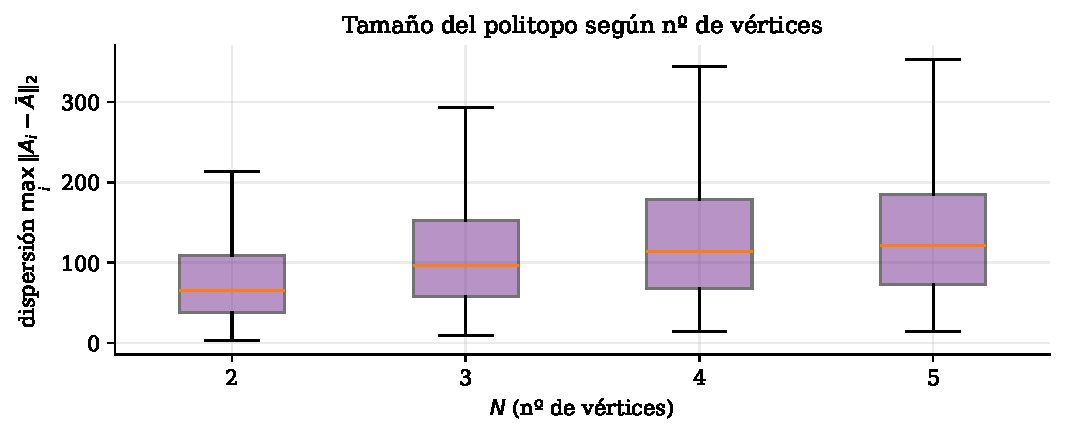
\includegraphics[width=0.82\linewidth]{fig6_dispersion.pdf}
  \caption{Tamaño del politopo $\max_i\lVert A_i-\bar A\rVert_2$ frente al número
  de vértices $N$. La incertidumbre crece con $N$.}
  \label{fig:dispersion}
\end{figure}

% --------------------------------------------------------------------
\subsection{El controlador y el sistema en lazo cerrado}
\label{sec:db-control}
% --------------------------------------------------------------------

``Lazo cerrado'' es el sistema \emph{con} el controlador conectado, gobernado por
$A_i+B_iK$. Verificamos numéricamente la etiqueta de la base recomputando los
autovalores de todos los vértices con su ganancia. El resultado es categórico:
\textbf{el $100\%$ de los $14\,000$ sistemas queda estable} (todos los
autovalores de todos los vértices con parte real negativa). No hay sistemas mal
etiquetados ni ganancias inconsistentes.

\paragraph{Estabilización ``al borde''.}
Lo más informativo es \emph{cómo} se estabiliza. La tasa de decaimiento lograda
$\alpha$ (Sec.~\ref{sec:db-conceptos}) —cuánto margen de estabilidad consigue el
controlador— se concentra masivamente junto a cero: su mediana es
$\alpha\approx 6.3\times10^{-4}$ y el $\mathbf{84.9\%}$ de los sistemas queda
\emph{casi marginal} ($\alpha<10^{-2}$), con sólo una minoría que alcanza
márgenes amplios ($\alpha_{95}=1.51$, máximo $10.6$). La distribución es
claramente \emph{bimodal} (Fig.~\ref{fig:decay}). Es decir, la ganancia de
referencia \emph{apenas} estabiliza: deja el modo dominante prácticamente sobre
la frontera de la inestabilidad.

\begin{figure}[t]
  \centering
  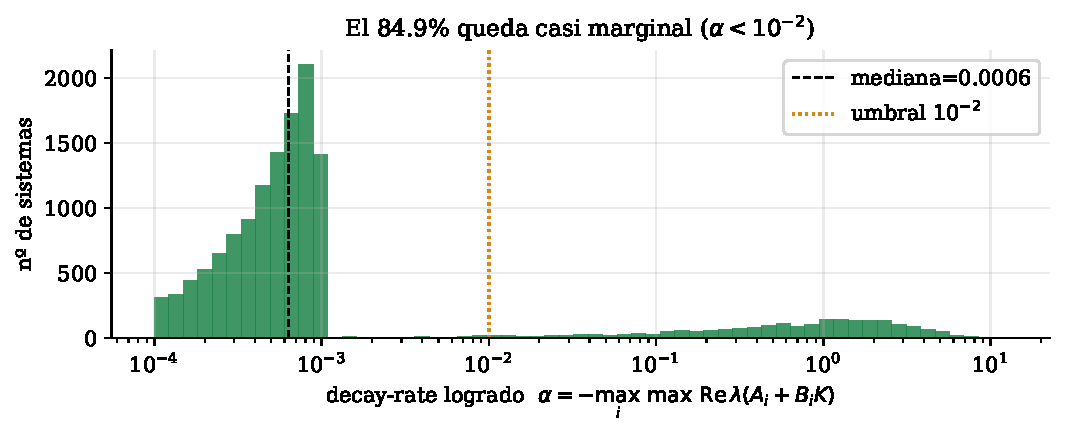
\includegraphics[width=\linewidth]{fig3_decay.pdf}
  \caption{Tasa de decaimiento lograda $\alpha$ (escala logarítmica). El
  $84.9\%$ de los sistemas queda casi marginal ($\alpha<10^{-2}$); una minoría
  exhibe márgenes grandes. La distribución es bimodal.}
  \label{fig:decay}
\end{figure}

Este comportamiento sugiere que las ganancias se construyeron buscando
\emph{cualquier} solución válida (factibilidad), no la más rápida. Lo respalda
un detalle: aunque el modo \emph{dominante} se aparca en la frontera, el resto de
los modos se empujan muy hacia la zona estable —la mediana de la parte real
sobre \emph{todos} los autovalores de lazo cerrado es $-21.4$. Visualmente, el
controlador ``refleja'' el espectro de la planta desde el semiplano inestable
(derecho) al estable (izquierdo), dejando un único modo lento que fija $\alpha$
(Fig.~\ref{fig:plano}).

\begin{figure}[t]
  \centering
  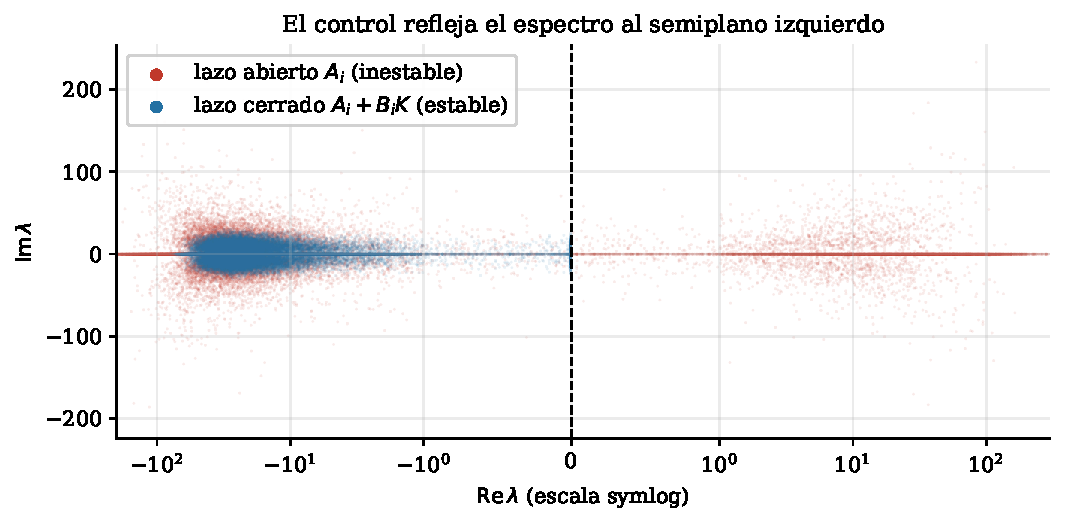
\includegraphics[width=\linewidth]{fig4_plano_complejo.pdf}
  \caption{Autovalores de los vértices en el plano complejo (eje horizontal en
  escala symlog). Sin control (rojo) la planta tiene autovalores en el semiplano
  derecho (inestables); con control (azul) todos pasan al semiplano izquierdo
  (estables), con el modo dominante pegado al eje.}
  \label{fig:plano}
\end{figure}

\paragraph{Esfuerzo de control.}
Lo ``caro'' que resulta controlar cada sistema se mide con $\lVert K\rVert_2$
(mediana $17.4$, máximo $98.1$). No es arbitrario: crece junto con el tamaño de
la planta ($\rho_{\text{Spearman}}=0.90$ frente a $\lVert A\rVert$), el tamaño
del politopo ($0.85$ frente a la dispersión) y la inestabilidad de lazo abierto
($0.63$); plantas más grandes e inestables exigen controladores más fuertes
(Fig.~\ref{fig:corr}). En cambio, la tasa de decaimiento $\alpha$ es
\emph{estadísticamente independiente} de todos los descriptores ($|\rho|\le0.04$
en todos los casos): el margen marginal no se debe a que el problema sea difícil,
sino a la forma en que se construyó la ganancia.

\begin{figure}[t]
  \centering
  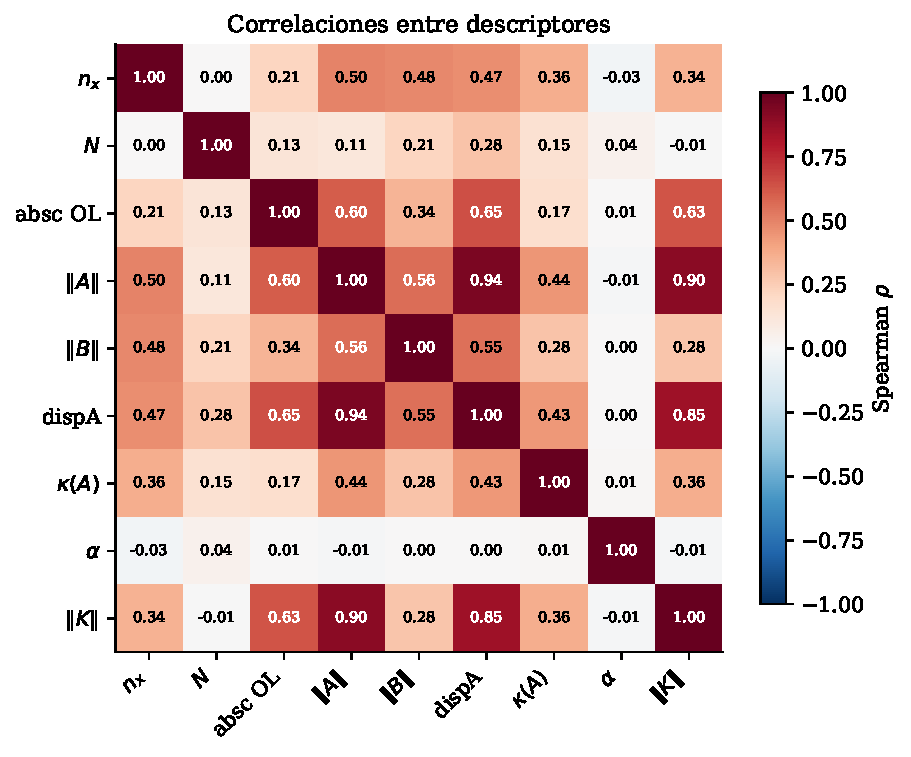
\includegraphics[width=0.78\linewidth]{fig8_correlaciones.pdf}
  \caption{Correlaciones de rango (Spearman) entre indicadores. El esfuerzo
  $\lVert K\rVert$ sigue al tamaño de la planta y del politopo; la tasa de
  decaimiento $\alpha$ no correlaciona con ningún indicador.}
  \label{fig:corr}
\end{figure}

% --------------------------------------------------------------------
\subsection{Calidad de los datos}
% --------------------------------------------------------------------

\begin{itemize}
  \item \textbf{Completitud:} sin valores faltantes en el soporte; las $28$
        celdas válidas están pobladas a $500/500$.
  \item \textbf{Validez de la etiqueta:} $100\%$ de los sistemas verificados como
        efectivamente estabilizados por su $K$ (todos los vértices estables).
  \item \textbf{Controlabilidad:} $100\%$ de los vértices controlables.
  \item \textbf{Duplicados:} no se detectaron sistemas repetidos.
  \item \textbf{Valores atípicos:} acotados y plausibles; la única cola de
        cuidado es el condicionamiento numérico ($0.39\%$ con $\kappa>10^4$),
        relevante para la estabilidad del cálculo más que para la validez del dato.
\end{itemize}

\begin{table}[t]
  \centering
  \caption{Resumen de indicadores sobre los $14\,000$ sistemas (datos crudos,
  sin normalizar).}
  \label{tab:resumen}
  \begin{tabular}{lrrr}
    \toprule
    Indicador & Mín. & Mediana & Máx. \\
    \midrule
    Abscisa espectral peor vértice (sin control) & $-17.9$ & $30.9$ & $832$ \\
    Tasa de decaimiento lograda $\alpha$         & $1.0\times10^{-4}$ & $6.3\times10^{-4}$ & $10.6$ \\
    $\max_i\lVert A_i\rVert_2$ (tamaño de la dinámica) & $12.2$ & $131$ & $1012$ \\
    $\max_i\lVert B_i\rVert_2$ (autoridad del control) & $0.74$ & $7.90$ & $16.8$ \\
    Dispersión del politopo (incertidumbre)      & $3.12$ & $97.5$ & $850$ \\
    Condición $\max_i\kappa(A_i)$                 & $1.44$ & $52.8$ & $5.7\times10^{5}$ \\
    Esfuerzo de control $\lVert K\rVert_2$        & $0.077$ & $17.4$ & $98.1$ \\
    \bottomrule
  \end{tabular}
\end{table}

% --------------------------------------------------------------------
\subsection{Implicaciones para el aprendizaje}
% --------------------------------------------------------------------

El análisis orienta varias decisiones de modelado:
%
\begin{enumerate}
  \item \textbf{Normalización imprescindible.} El rango de tamaños de $\lVert
        A\rVert$ (tres órdenes de magnitud) hace inviable alimentar las matrices
        crudas a la red; la reescala por $\gamma$ es necesaria para que el
        aprendizaje esté bien condicionado.
  \item \textbf{Invarianzas a aprovechar.} Un sistema es un \emph{conjunto} de
        vértices $\{(A_i,B_i)\}$ cuyo orden no importa y cuya cantidad $N$ varía,
        pero el certificado $K$ es común; esto motiva un codificador invariante
        al orden y a la cantidad de vértices (y, análogamente, al número de
        actuadores $n_u$).
  \item \textbf{Evaluar separado por $N$.} Como la incertidumbre crece con el
        número de vértices, conviene reportar el desempeño desglosado por $N$.
  \item \textbf{Sobre la señal de entrenamiento.} La ganancia de referencia es
        casi marginal y su $\alpha$ no aporta información sobre el sistema; esto
        respalda usar un objetivo \emph{auto-supervisado} —estabilizar con un
        margen $\alpha$ prescrito— en lugar de copiar directamente la $K$
        almacenada.
\end{enumerate}

%  Requiere: graphicx, booktabs, amsmath, amssymb
%  \graphicspath{{figuras/}}  % o ajusta la ruta a tus figuras
% =====================================================================

\section{Caracterización de la base de datos}
\label{sec:analisis-db}

% --------------------------------------------------------------------
\subsection{Propósito y estructura}
% --------------------------------------------------------------------

La base de datos \texttt{DB\_ssf\_RS\_500\_c.mat} es el conjunto de
entrenamiento del modelo. Cada muestra describe un \emph{sistema dinámico
incierto} junto con un controlador que lo estabiliza. Conviene fijar primero la
intuición de qué es cada cosa antes de cuantificarla.

Un \textbf{sistema lineal} modela cómo evoluciona en el tiempo un vector de
estado $x(t)\in\mathbb{R}^{n_x}$ (las variables internas del proceso) cuando se
le aplica una señal de control $u(t)\in\mathbb{R}^{n_u}$:
%
\begin{equation}
  \dot{x}(t) = A\,x(t) + B\,u(t).
  \label{eq:lti}
\end{equation}
%
La matriz $A$ codifica la \emph{dinámica propia} del sistema (cómo se influyen
entre sí las variables si no hiciéramos nada), y $B$ describe \emph{cómo entra
el control} en esa dinámica. El número $n_x$ es el \emph{orden} (cuántas
variables de estado) y $n_u$ es el número de \emph{actuadores} (cuántas
perillas de control independientes hay).

En la práctica el sistema no se conoce con exactitud: hay incertidumbre en sus
parámetros. Se modela esa incertidumbre con un \textbf{politopo}, es decir, una
familia de sistemas posibles obtenida ``mezclando'' $N$ casos extremos
conocidos —los \emph{vértices} $(A_i,B_i)$— en todas las proporciones
convexas:
%
\begin{equation}
  \bigl(A(\theta),B(\theta)\bigr)=\sum_{i=1}^{N}\theta_i\,(A_i,B_i),
  \qquad \theta_i\ge 0,\ \textstyle\sum_i\theta_i=1.
  \label{eq:politopo}
\end{equation}
%
Intuitivamente, el sistema real es \emph{algún} punto dentro de la envolvente
convexa de esos $N$ vértices, pero no sabemos cuál; un controlador
\emph{robusto} debe funcionar para todos a la vez. Esto es análogo, en
términos de computación, a exigir una garantía en el \emph{peor caso} sobre un
conjunto acotado de entradas posibles.

Cada muestra de la base es por tanto una terna: el conjunto de vértices
$\{A_i\}$, el conjunto $\{B_i\}$, y una \textbf{ganancia} $K\in\mathbb{R}^{n_u\times
n_x}$ que define el controlador por realimentación de estado $u(t)=K\,x(t)$ —una
única $K$ que estabiliza todo el politopo (Tabla~\ref{tab:esquema}). La etiqueta
\texttt{RS} (\emph{robustly stabilizable}) indica que el sistema admite tal
ganancia robusta.\footnote{\textbf{Procedencia (por confirmar con el autor de la
base):} la evidencia empírica (Sec.~\ref{sec:db-control}) es consistente con que
cada $K$ se obtuvo resolviendo un problema de factibilidad (una LMI de
estabilizabilidad cuadrática), sin optimizar la rapidez de la respuesta. Falta
confirmar cómo se generaron los vértices $(A_i,B_i)$.}

\begin{table}[t]
  \centering
  \caption{Esquema de la base de datos. Cada sistema es un politopo de $N$
  vértices con una ganancia robusta $K$.}
  \label{tab:esquema}
  \begin{tabular}{llll}
    \toprule
    Campo & Símbolo & Forma & Descripción \\
    \midrule
    \texttt{A} & $\{A_i\}_{i=1}^N$ & $N\times(n_x\!\times\! n_x)$ & Dinámica propia de cada vértice \\
    \texttt{B} & $\{B_i\}_{i=1}^N$ & $N\times(n_x\!\times\! n_u)$ & Entrada de control de cada vértice \\
    \texttt{K} & $K$               & $n_u\times n_x$             & Ganancia del controlador (común) \\
    \midrule
    \multicolumn{4}{l}{$n_x\in\{2,3,4,5\}$\quad $n_u\in\{1,2\}$\quad $N\in\{2,3,4,5\}$\quad $500$ casos/celda} \\
    \bottomrule
  \end{tabular}
\end{table}

% --------------------------------------------------------------------
\subsection{Cómo se mide un sistema y su estabilidad}
\label{sec:db-conceptos}
% --------------------------------------------------------------------

Para caracterizar la base usamos un puñado de indicadores numéricos. Como el
lector no tiene por qué venir de teoría de control, los explicamos aquí en
lenguaje llano; la Tabla~\ref{tab:glosario} los resume.

\paragraph{Estabilidad y autovalores.}
La pregunta central sobre un sistema es si es \emph{estable}: si lo perturbamos,
¿vuelve al equilibrio o se dispara? Para un sistema lineal
$\dot{x}=Ax$, la respuesta la dan los \textbf{autovalores} de $A$. Toda
solución es una combinación de ``modos'' de la forma $e^{\lambda t}$, donde
$\lambda=a+bi$ es un autovalor. Su \emph{parte real} $a=\operatorname{Re}\lambda$
controla la magnitud ($e^{at}$ crece si $a>0$ y decae si $a<0$) y su parte
imaginaria $b$ controla la oscilación. Por tanto:
%
\begin{center}
  \emph{el sistema es estable} $\iff$ \emph{todos} sus autovalores cumplen
  $\operatorname{Re}\lambda<0$.
\end{center}
%
En el plano complejo, esto es ``todos los autovalores en el semiplano
izquierdo''.

\paragraph{Abscisa espectral: el modo que decide.}
No hace falta mirar todos los autovalores: basta el \emph{peor}. La
\textbf{abscisa espectral} es el mayor de las partes reales,
$\max\operatorname{Re}\lambda(A)$. Es el modo que crece más rápido (o decae más
lento) y, por sí solo, decide la estabilidad: si la abscisa es negativa, todos
los modos decaen; si es positiva, al menos uno explota. Un valor de, por
ejemplo, $832$ significa que el modo dominante crece como $e^{832\,t}$: una
inestabilidad extremadamente violenta. Lo usamos como \emph{medida relativa de
qué tan inestable} es una planta (no tiene unidades físicas porque los sistemas
son sintéticos).

\paragraph{Los dos ``máximos''.}
En las fórmulas aparecen \emph{dos} máximos anidados, y conviene separarlos:
%
\begin{equation*}
  \underbrace{\max_{i=1,\dots,N}}_{\text{(2) peor \emph{vértice}}}
  \ \underbrace{\max\,\operatorname{Re}\,\lambda(A_i)}_{\text{(1) peor \emph{modo} de ese vértice}}.
\end{equation*}
%
El máximo interno (1) recorre los autovalores de \emph{un} vértice y se queda
con su modo dominante (la abscisa espectral de $A_i$). El máximo externo (2)
recorre los $N$ vértices del politopo y se queda con el más desfavorable. La
combinación es la lectura de \emph{peor caso}: ``de toda la familia de sistemas
posibles, ¿qué tan mal se comporta el peor de ellos?''.

\paragraph{Norma de una matriz: su ``tamaño''.}
La norma espectral $\lVert A\rVert_2$ mide cuánto puede \emph{amplificar} esa
matriz a un vector (formalmente, su mayor valor singular). Es una medida del
``tamaño'' o la fuerza de la dinámica: una $\lVert A\rVert_2$ grande indica
acoplamientos internos intensos. Reportamos $\max_i\lVert A_i\rVert_2$, el
tamaño del vértice más grande del politopo.

\paragraph{Tasa de decaimiento $\alpha$: el margen de seguridad.}
Una vez cerrado el lazo con el controlador, la matriz que gobierna la dinámica
pasa a ser $A_i+B_iK$. Su abscisa espectral, cambiada de signo, es la
\textbf{tasa de decaimiento}
$\alpha=-\max_i\max\operatorname{Re}\lambda(A_i+B_iK)$. Mide \emph{qué tan
rápido} se extingue la peor respuesta: $\alpha>0$ garantiza estabilidad, y
cuanto mayor sea $\alpha$, más rápido y con más margen vuelve el sistema al
equilibrio. Un $\alpha\approx0$ significa ``estable, pero al borde'': el sistema
apenas se sostiene sobre la frontera de la inestabilidad.

\paragraph{Otros indicadores.}
La \emph{dispersión del politopo} $\max_i\lVert A_i-\bar A\rVert_2$ (con $\bar A$
el promedio de los vértices) mide qué tan distintos son los vértices entre sí,
es decir, cuánta incertidumbre hay. El \emph{número de condición} $\kappa(A_i)$
mide la sensibilidad numérica de la matriz (valores altos anticipan problemas de
precisión). El \emph{esfuerzo de control} $\lVert K\rVert_2$ mide qué tan
``agresivo'' es el controlador.

\begin{table}[t]
  \centering
  \caption{Glosario de indicadores usados en el análisis.}
  \label{tab:glosario}
  \small
  \begin{tabular}{p{3.0cm}p{3.4cm}p{6.6cm}}
    \toprule
    Indicador & En palabras simples & Un valor alto significa\dots \\
    \midrule
    Abscisa espectral (lazo abierto)\newline $\max_i\max\operatorname{Re}\lambda(A_i)$
      & Rapidez del modo más inestable del peor vértice
      & Planta muy inestable: sin control, se dispara muy rápido. \\
    Tasa de decaimiento\newline $\alpha=-\max_i\max\operatorname{Re}\lambda(A_i+B_iK)$
      & Qué tan rápido se calma el sistema ya controlado
      & Más margen de estabilidad; $\alpha\approx0$ = estable al borde. \\
    Norma $\max_i\lVert A_i\rVert_2$
      & ``Tamaño''/fuerza de la dinámica propia
      & Acoplamientos internos intensos. \\
    Norma $\max_i\lVert B_i\rVert_2$
      & Cuánto influye el control en el estado
      & Actuadores con mucha autoridad. \\
    Dispersión del politopo\newline $\max_i\lVert A_i-\bar A\rVert_2$
      & Qué tan distintos son los vértices
      & Más incertidumbre que cubrir con una sola $K$. \\
    Condición $\kappa(A_i)$
      & Sensibilidad numérica de la matriz
      & Riesgo de imprecisión numérica. \\
    Esfuerzo $\lVert K\rVert_2$
      & Qué tan ``fuerte'' es el controlador
      & Acción de control más agresiva. \\
    \bottomrule
  \end{tabular}
\end{table}

% --------------------------------------------------------------------
\subsection{Cobertura y diseño experimental}
% --------------------------------------------------------------------

El archivo organiza las muestras en un arreglo de cuatro índices,
$\texttt{BASE}[\,n_x,\,n_u,\,N,\,\text{caso}\,]$, de forma nominal
$5\times 2\times 5\times 500$. La malla está poblada parcialmente: el orden
mínimo depende del número de actuadores ($n_u{=}1\Rightarrow n_x\in\{2,\dots,5\}$;
$n_u{=}2\Rightarrow n_x\in\{3,4,5\}$) y siempre $N\ge 2$. De las $25\,000$
posiciones nominales sólo $28$ están ocupadas, con exactamente $500$ casos cada
una: en total $\mathbf{14\,000}$ sistemas ($8\,000$ con $n_u{=}1$ y $6\,000$ con
$n_u{=}2$).

La base sigue así un \emph{diseño factorial completo y perfectamente
balanceado} sobre los factores $(n_x, n_u, N)$ admisibles
(Fig.~\ref{fig:cobertura}): las $28$ combinaciones válidas aparecen con la misma
cantidad de ejemplos ($500$), sin celdas faltantes ni sobre-representadas. Este
balance es deseable para el aprendizaje: evita que el modelo privilegie una
configuración por mero desbalance de frecuencia, y permite reportar métricas
separadas por $N$ y por $n_x$ sin correcciones.

\begin{figure}[t]
  \centering
  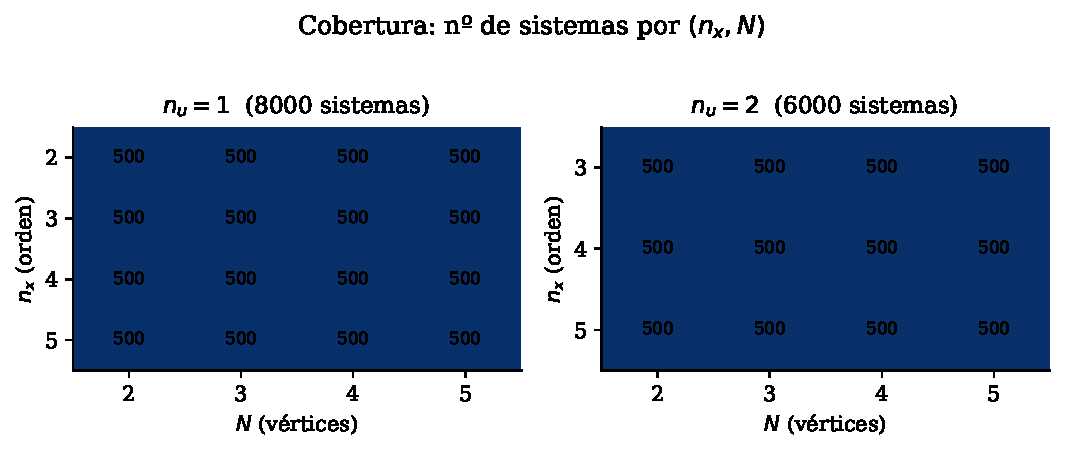
\includegraphics[width=\linewidth]{fig1_cobertura.pdf}
  \caption{Cobertura factorial: número de sistemas por $(n_x,N)$, separado por
  número de actuadores $n_u$. El soporte está completamente balanceado a $500$
  sistemas por celda.}
  \label{fig:cobertura}
\end{figure}

% --------------------------------------------------------------------
\subsection{La planta sin control (lazo abierto)}
\label{sec:db-ol}
% --------------------------------------------------------------------

``Lazo abierto'' se refiere al sistema \emph{sin} controlador. Las plantas de la
base son \emph{difíciles}: el $\mathbf{98.8\%}$ es inestable en lazo abierto
(al menos un vértice tiene un autovalor con parte real positiva), y sólo el
$1.2\%$ sería estable por sí solo. La abscisa espectral del peor vértice
(la rapidez del modo más inestable, ver Sec.~\ref{sec:db-conceptos}) tiene
mediana $30.9$ y llega hasta $\sim\!832$ (Fig.~\ref{fig:estabilidad}). En otras
palabras, la base no contiene casos triviales: el controlador debe
\emph{crear} la estabilidad, no sólo conservarla.

\begin{figure}[t]
  \centering
  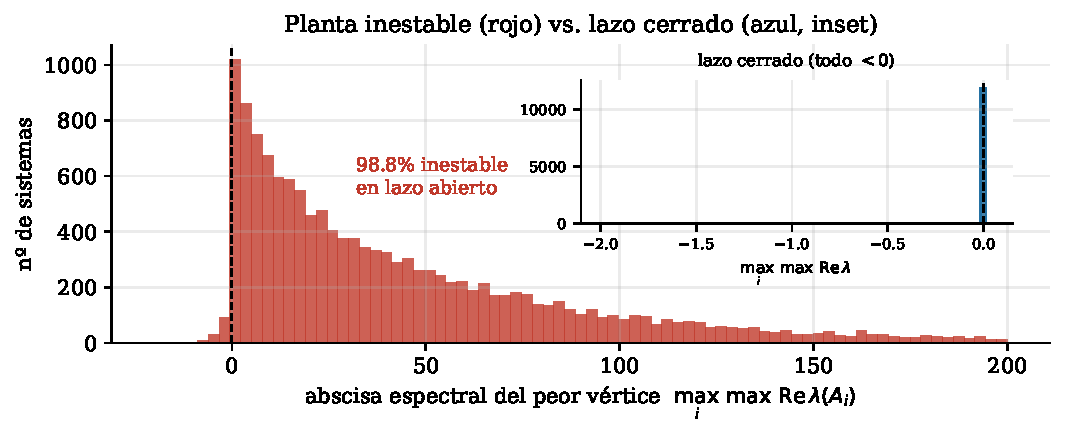
\includegraphics[width=\linewidth]{fig2_estabilidad.pdf}
  \caption{Abscisa espectral del peor vértice. Sin control la planta es
  inestable (rojo, parte real $>0$) en el $98.8\%$ de los casos; con la ganancia
  $K$ el lazo cerrado es estable en el $100\%$ (inset azul, todos $<0$).}
  \label{fig:estabilidad}
\end{figure}

En cuanto al ``tamaño'' de la dinámica (Fig.~\ref{fig:normas}), los descriptores
tienen un rango muy amplio: $\max_i\lVert A_i\rVert_2$ va de $12$ a $1012$
(mediana $131$) y crece de forma marcada con el orden $n_x$, mientras que
$\max_i\lVert B_i\rVert_2$ se mantiene acotado en $[0.74,\,16.8]$. Esta
disparidad de escalas —tres órdenes de magnitud en $\lVert A\rVert$— es
justamente la que obliga a \emph{normalizar} los datos antes de entrenar: cada
politopo se reescala dividiéndolo por su entrada de mayor magnitud,
$\gamma=\max(\max|A|,\max|B|)$, de modo que todas las cifras queden en
$[-1,1]$ y los sistemas sean comparables entre sí (esta reescala no cambia el
signo de los autovalores —y por tanto no afecta la estabilidad— aunque sí divide
la tasa de decaimiento por $\gamma$).

\begin{figure}[t]
  \centering
  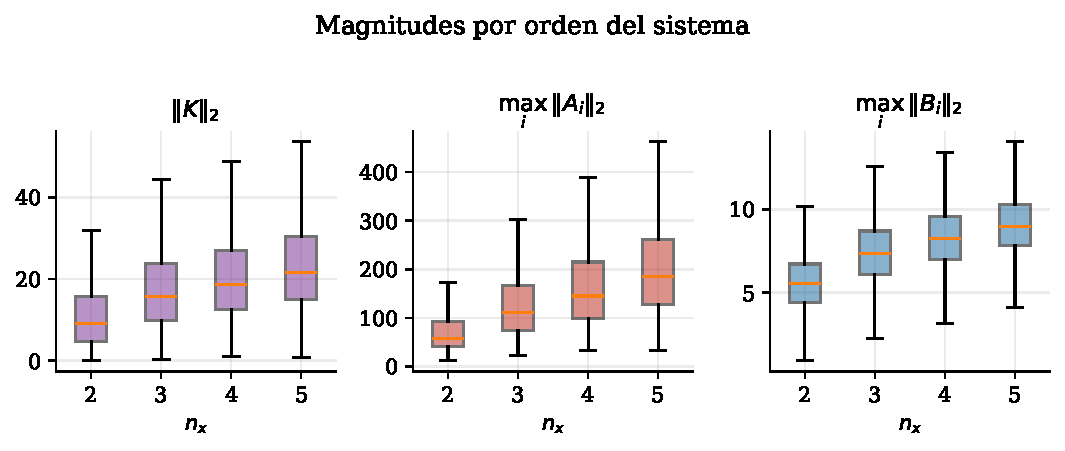
\includegraphics[width=\linewidth]{fig5_normas.pdf}
  \caption{Distribución del esfuerzo de control $\lVert K\rVert_2$ y de los
  tamaños $\max_i\lVert A_i\rVert_2$ y $\max_i\lVert B_i\rVert_2$, según el orden
  $n_x$. Ambos crecen con el orden del sistema.}
  \label{fig:normas}
\end{figure}

\paragraph{¿Se puede controlar? Controlabilidad y condicionamiento.}
Un requisito previo para que exista una ganancia estabilizante es que el sistema
sea \emph{controlable}: que desde la entrada se pueda influir en todas las
direcciones del estado. Esto se cumple en el $100\%$ de los vértices de todos
los sistemas. El número de condición de las matrices es benigno en general
($\kappa(A_i)$ con mediana $53$), con una cola pesada: un $0.39\%$ de los
sistemas supera $\kappa>10^4$, con casos extremos de hasta $5.7\times10^5$
(Fig.~\ref{fig:cond}); estos son los sistemas numéricamente delicados durante el
entrenamiento.

\begin{figure}[t]
  \centering
  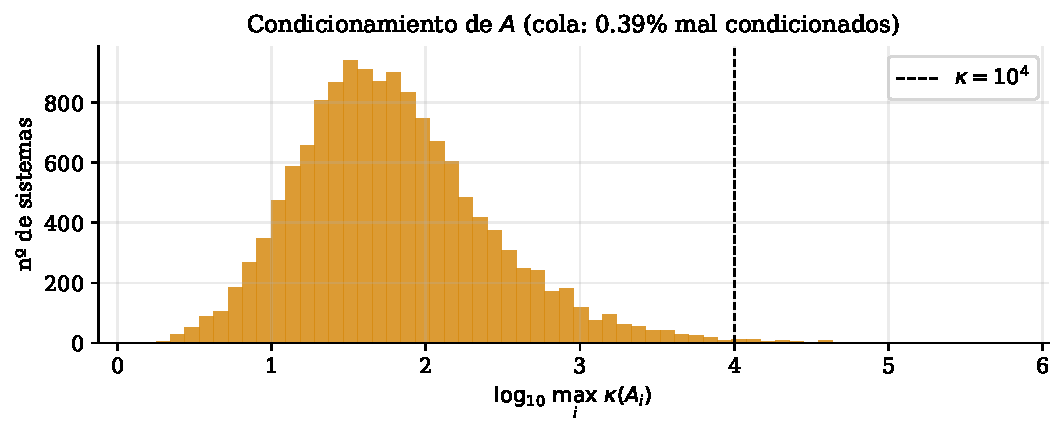
\includegraphics[width=0.82\linewidth]{fig7_condicionamiento.pdf}
  \caption{Número de condición $\max_i\kappa(A_i)$ (escala $\log_{10}$). La gran
  mayoría está bien condicionada; una cola del $0.39\%$ supera $\kappa=10^4$.}
  \label{fig:cond}
\end{figure}

% --------------------------------------------------------------------
\subsection{Tamaño de la incertidumbre (geometría del politopo)}
% --------------------------------------------------------------------

¿Qué tan ``grande'' es la incertidumbre de cada sistema? Lo medimos con la
dispersión de los vértices respecto a su promedio,
$\max_i\lVert A_i-\bar A\rVert_2$: si los vértices son muy parecidos entre sí, el
politopo es pequeño (poca incertidumbre); si son muy distintos, es grande. Su
mediana es $97.5$ y crece de forma sistemática con el número de vértices $N$
(Fig.~\ref{fig:dispersion}): más vértices implican politopos más amplios y, por
tanto, una incertidumbre más severa que la \emph{misma} ganancia $K$ debe cubrir
a la vez. Esto convierte a $N$ en un eje natural de dificultad y motiva evaluar
el modelo \emph{separado por $N$}.

\begin{figure}[t]
  \centering
  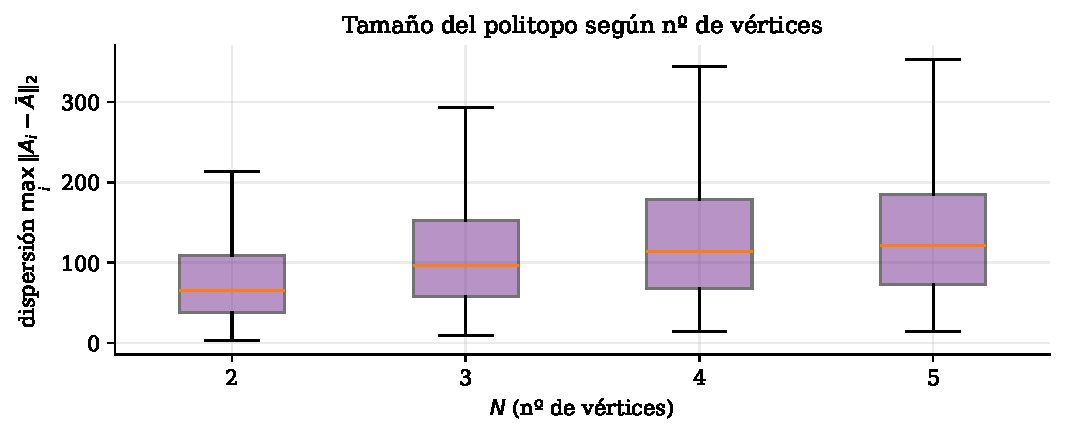
\includegraphics[width=0.82\linewidth]{fig6_dispersion.pdf}
  \caption{Tamaño del politopo $\max_i\lVert A_i-\bar A\rVert_2$ frente al número
  de vértices $N$. La incertidumbre crece con $N$.}
  \label{fig:dispersion}
\end{figure}

% --------------------------------------------------------------------
\subsection{El controlador y el sistema en lazo cerrado}
\label{sec:db-control}
% --------------------------------------------------------------------

``Lazo cerrado'' es el sistema \emph{con} el controlador conectado, gobernado por
$A_i+B_iK$. Verificamos numéricamente la etiqueta de la base recomputando los
autovalores de todos los vértices con su ganancia. El resultado es categórico:
\textbf{el $100\%$ de los $14\,000$ sistemas queda estable} (todos los
autovalores de todos los vértices con parte real negativa). No hay sistemas mal
etiquetados ni ganancias inconsistentes.

\paragraph{Estabilización ``al borde''.}
Lo más informativo es \emph{cómo} se estabiliza. La tasa de decaimiento lograda
$\alpha$ (Sec.~\ref{sec:db-conceptos}) —cuánto margen de estabilidad consigue el
controlador— se concentra masivamente junto a cero: su mediana es
$\alpha\approx 6.3\times10^{-4}$ y el $\mathbf{84.9\%}$ de los sistemas queda
\emph{casi marginal} ($\alpha<10^{-2}$), con sólo una minoría que alcanza
márgenes amplios ($\alpha_{95}=1.51$, máximo $10.6$). La distribución es
claramente \emph{bimodal} (Fig.~\ref{fig:decay}). Es decir, la ganancia de
referencia \emph{apenas} estabiliza: deja el modo dominante prácticamente sobre
la frontera de la inestabilidad.

\begin{figure}[t]
  \centering
  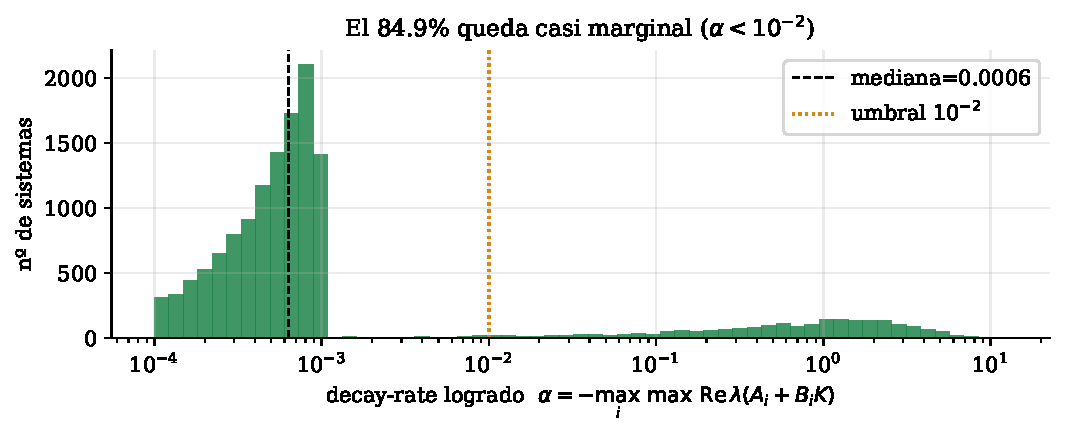
\includegraphics[width=\linewidth]{fig3_decay.pdf}
  \caption{Tasa de decaimiento lograda $\alpha$ (escala logarítmica). El
  $84.9\%$ de los sistemas queda casi marginal ($\alpha<10^{-2}$); una minoría
  exhibe márgenes grandes. La distribución es bimodal.}
  \label{fig:decay}
\end{figure}

Este comportamiento sugiere que las ganancias se construyeron buscando
\emph{cualquier} solución válida (factibilidad), no la más rápida. Lo respalda
un detalle: aunque el modo \emph{dominante} se aparca en la frontera, el resto de
los modos se empujan muy hacia la zona estable —la mediana de la parte real
sobre \emph{todos} los autovalores de lazo cerrado es $-21.4$. Visualmente, el
controlador ``refleja'' el espectro de la planta desde el semiplano inestable
(derecho) al estable (izquierdo), dejando un único modo lento que fija $\alpha$
(Fig.~\ref{fig:plano}).

\begin{figure}[t]
  \centering
  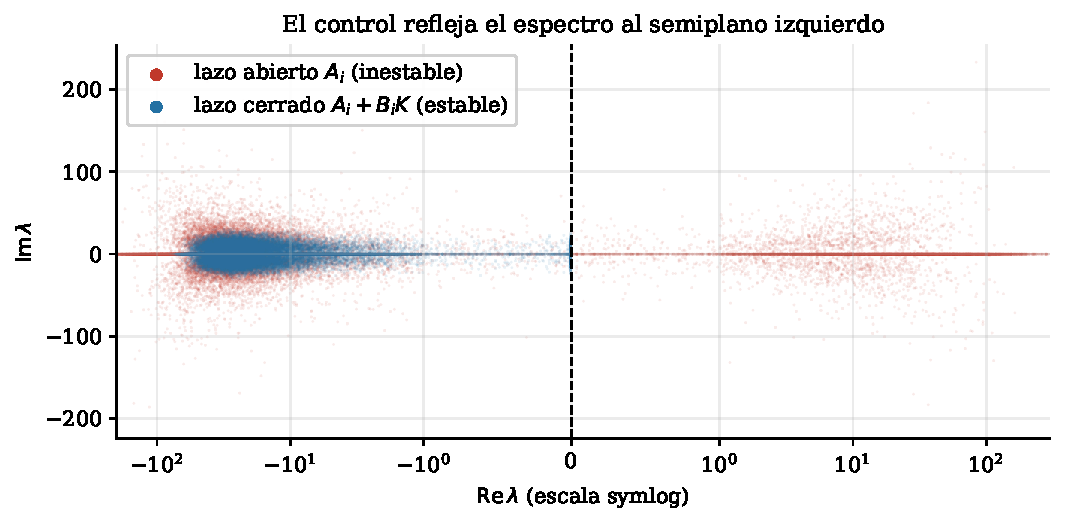
\includegraphics[width=\linewidth]{fig4_plano_complejo.pdf}
  \caption{Autovalores de los vértices en el plano complejo (eje horizontal en
  escala symlog). Sin control (rojo) la planta tiene autovalores en el semiplano
  derecho (inestables); con control (azul) todos pasan al semiplano izquierdo
  (estables), con el modo dominante pegado al eje.}
  \label{fig:plano}
\end{figure}

\paragraph{Esfuerzo de control.}
Lo ``caro'' que resulta controlar cada sistema se mide con $\lVert K\rVert_2$
(mediana $17.4$, máximo $98.1$). No es arbitrario: crece junto con el tamaño de
la planta ($\rho_{\text{Spearman}}=0.90$ frente a $\lVert A\rVert$), el tamaño
del politopo ($0.85$ frente a la dispersión) y la inestabilidad de lazo abierto
($0.63$); plantas más grandes e inestables exigen controladores más fuertes
(Fig.~\ref{fig:corr}). En cambio, la tasa de decaimiento $\alpha$ es
\emph{estadísticamente independiente} de todos los descriptores ($|\rho|\le0.04$
en todos los casos): el margen marginal no se debe a que el problema sea difícil,
sino a la forma en que se construyó la ganancia.

\begin{figure}[t]
  \centering
  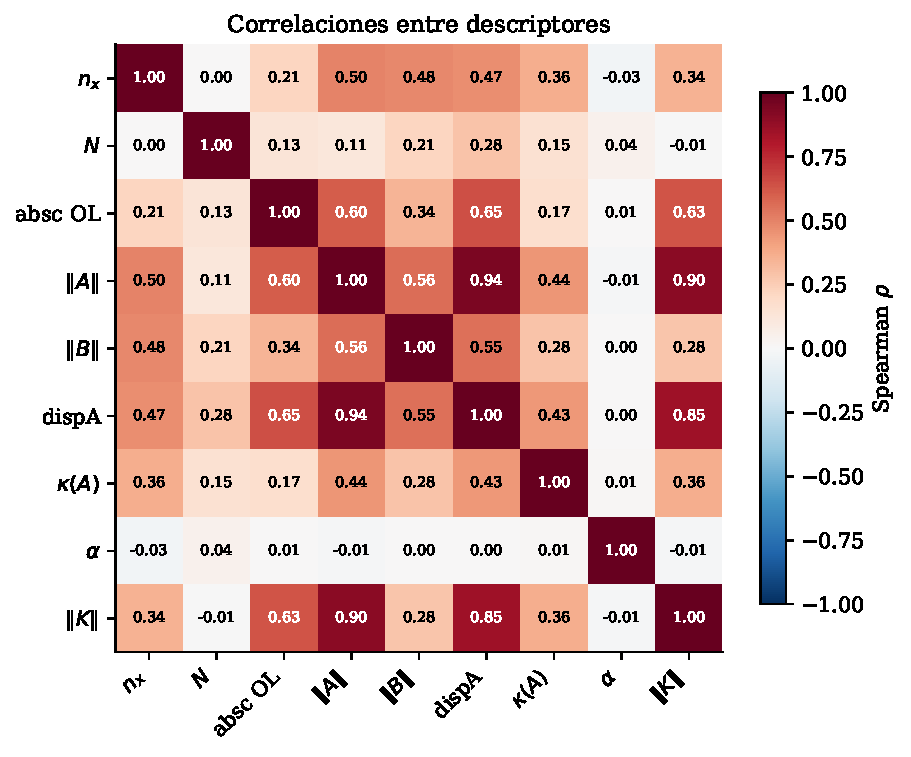
\includegraphics[width=0.78\linewidth]{fig8_correlaciones.pdf}
  \caption{Correlaciones de rango (Spearman) entre indicadores. El esfuerzo
  $\lVert K\rVert$ sigue al tamaño de la planta y del politopo; la tasa de
  decaimiento $\alpha$ no correlaciona con ningún indicador.}
  \label{fig:corr}
\end{figure}

% --------------------------------------------------------------------
\subsection{Calidad de los datos}
% --------------------------------------------------------------------

\begin{itemize}
  \item \textbf{Completitud:} sin valores faltantes en el soporte; las $28$
        celdas válidas están pobladas a $500/500$.
  \item \textbf{Validez de la etiqueta:} $100\%$ de los sistemas verificados como
        efectivamente estabilizados por su $K$ (todos los vértices estables).
  \item \textbf{Controlabilidad:} $100\%$ de los vértices controlables.
  \item \textbf{Duplicados:} no se detectaron sistemas repetidos.
  \item \textbf{Valores atípicos:} acotados y plausibles; la única cola de
        cuidado es el condicionamiento numérico ($0.39\%$ con $\kappa>10^4$),
        relevante para la estabilidad del cálculo más que para la validez del dato.
\end{itemize}

\begin{table}[t]
  \centering
  \caption{Resumen de indicadores sobre los $14\,000$ sistemas (datos crudos,
  sin normalizar).}
  \label{tab:resumen}
  \begin{tabular}{lrrr}
    \toprule
    Indicador & Mín. & Mediana & Máx. \\
    \midrule
    Abscisa espectral peor vértice (sin control) & $-17.9$ & $30.9$ & $832$ \\
    Tasa de decaimiento lograda $\alpha$         & $1.0\times10^{-4}$ & $6.3\times10^{-4}$ & $10.6$ \\
    $\max_i\lVert A_i\rVert_2$ (tamaño de la dinámica) & $12.2$ & $131$ & $1012$ \\
    $\max_i\lVert B_i\rVert_2$ (autoridad del control) & $0.74$ & $7.90$ & $16.8$ \\
    Dispersión del politopo (incertidumbre)      & $3.12$ & $97.5$ & $850$ \\
    Condición $\max_i\kappa(A_i)$                 & $1.44$ & $52.8$ & $5.7\times10^{5}$ \\
    Esfuerzo de control $\lVert K\rVert_2$        & $0.077$ & $17.4$ & $98.1$ \\
    \bottomrule
  \end{tabular}
\end{table}

% --------------------------------------------------------------------
\subsection{Implicaciones para el aprendizaje}
% --------------------------------------------------------------------

El análisis orienta varias decisiones de modelado:
%
\begin{enumerate}
  \item \textbf{Normalización imprescindible.} El rango de tamaños de $\lVert
        A\rVert$ (tres órdenes de magnitud) hace inviable alimentar las matrices
        crudas a la red; la reescala por $\gamma$ es necesaria para que el
        aprendizaje esté bien condicionado.
  \item \textbf{Invarianzas a aprovechar.} Un sistema es un \emph{conjunto} de
        vértices $\{(A_i,B_i)\}$ cuyo orden no importa y cuya cantidad $N$ varía,
        pero el certificado $K$ es común; esto motiva un codificador invariante
        al orden y a la cantidad de vértices (y, análogamente, al número de
        actuadores $n_u$).
  \item \textbf{Evaluar separado por $N$.} Como la incertidumbre crece con el
        número de vértices, conviene reportar el desempeño desglosado por $N$.
  \item \textbf{Sobre la señal de entrenamiento.} La ganancia de referencia es
        casi marginal y su $\alpha$ no aporta información sobre el sistema; esto
        respalda usar un objetivo \emph{auto-supervisado} —estabilizar con un
        margen $\alpha$ prescrito— en lugar de copiar directamente la $K$
        almacenada.
\end{enumerate}

%  Requiere: graphicx, booktabs, amsmath, amssymb
%  \graphicspath{{figuras/}}  % o ajusta la ruta a tus figuras
% =====================================================================

\section{Caracterización de la base de datos}
\label{sec:analisis-db}

% --------------------------------------------------------------------
\subsection{Propósito y estructura}
% --------------------------------------------------------------------

La base de datos \texttt{DB\_ssf\_RS\_500\_c.mat} es el conjunto de
entrenamiento del modelo. Cada muestra describe un \emph{sistema dinámico
incierto} junto con un controlador que lo estabiliza. Conviene fijar primero la
intuición de qué es cada cosa antes de cuantificarla.

Un \textbf{sistema lineal} modela cómo evoluciona en el tiempo un vector de
estado $x(t)\in\mathbb{R}^{n_x}$ (las variables internas del proceso) cuando se
le aplica una señal de control $u(t)\in\mathbb{R}^{n_u}$:
%
\begin{equation}
  \dot{x}(t) = A\,x(t) + B\,u(t).
  \label{eq:lti}
\end{equation}
%
La matriz $A$ codifica la \emph{dinámica propia} del sistema (cómo se influyen
entre sí las variables si no hiciéramos nada), y $B$ describe \emph{cómo entra
el control} en esa dinámica. El número $n_x$ es el \emph{orden} (cuántas
variables de estado) y $n_u$ es el número de \emph{actuadores} (cuántas
perillas de control independientes hay).

En la práctica el sistema no se conoce con exactitud: hay incertidumbre en sus
parámetros. Se modela esa incertidumbre con un \textbf{politopo}, es decir, una
familia de sistemas posibles obtenida ``mezclando'' $N$ casos extremos
conocidos —los \emph{vértices} $(A_i,B_i)$— en todas las proporciones
convexas:
%
\begin{equation}
  \bigl(A(\theta),B(\theta)\bigr)=\sum_{i=1}^{N}\theta_i\,(A_i,B_i),
  \qquad \theta_i\ge 0,\ \textstyle\sum_i\theta_i=1.
  \label{eq:politopo}
\end{equation}
%
Intuitivamente, el sistema real es \emph{algún} punto dentro de la envolvente
convexa de esos $N$ vértices, pero no sabemos cuál; un controlador
\emph{robusto} debe funcionar para todos a la vez. Esto es análogo, en
términos de computación, a exigir una garantía en el \emph{peor caso} sobre un
conjunto acotado de entradas posibles.

Cada muestra de la base es por tanto una terna: el conjunto de vértices
$\{A_i\}$, el conjunto $\{B_i\}$, y una \textbf{ganancia} $K\in\mathbb{R}^{n_u\times
n_x}$ que define el controlador por realimentación de estado $u(t)=K\,x(t)$ —una
única $K$ que estabiliza todo el politopo (Tabla~\ref{tab:esquema}). La etiqueta
\texttt{RS} (\emph{robustly stabilizable}) indica que el sistema admite tal
ganancia robusta.\footnote{\textbf{Procedencia (por confirmar con el autor de la
base):} la evidencia empírica (Sec.~\ref{sec:db-control}) es consistente con que
cada $K$ se obtuvo resolviendo un problema de factibilidad (una LMI de
estabilizabilidad cuadrática), sin optimizar la rapidez de la respuesta. Falta
confirmar cómo se generaron los vértices $(A_i,B_i)$.}

\begin{table}[t]
  \centering
  \caption{Esquema de la base de datos. Cada sistema es un politopo de $N$
  vértices con una ganancia robusta $K$.}
  \label{tab:esquema}
  \begin{tabular}{llll}
    \toprule
    Campo & Símbolo & Forma & Descripción \\
    \midrule
    \texttt{A} & $\{A_i\}_{i=1}^N$ & $N\times(n_x\!\times\! n_x)$ & Dinámica propia de cada vértice \\
    \texttt{B} & $\{B_i\}_{i=1}^N$ & $N\times(n_x\!\times\! n_u)$ & Entrada de control de cada vértice \\
    \texttt{K} & $K$               & $n_u\times n_x$             & Ganancia del controlador (común) \\
    \midrule
    \multicolumn{4}{l}{$n_x\in\{2,3,4,5\}$\quad $n_u\in\{1,2\}$\quad $N\in\{2,3,4,5\}$\quad $500$ casos/celda} \\
    \bottomrule
  \end{tabular}
\end{table}

% --------------------------------------------------------------------
\subsection{Cómo se mide un sistema y su estabilidad}
\label{sec:db-conceptos}
% --------------------------------------------------------------------

Para caracterizar la base usamos un puñado de indicadores numéricos. Como el
lector no tiene por qué venir de teoría de control, los explicamos aquí en
lenguaje llano; la Tabla~\ref{tab:glosario} los resume.

\paragraph{Estabilidad y autovalores.}
La pregunta central sobre un sistema es si es \emph{estable}: si lo perturbamos,
¿vuelve al equilibrio o se dispara? Para un sistema lineal
$\dot{x}=Ax$, la respuesta la dan los \textbf{autovalores} de $A$. Toda
solución es una combinación de ``modos'' de la forma $e^{\lambda t}$, donde
$\lambda=a+bi$ es un autovalor. Su \emph{parte real} $a=\operatorname{Re}\lambda$
controla la magnitud ($e^{at}$ crece si $a>0$ y decae si $a<0$) y su parte
imaginaria $b$ controla la oscilación. Por tanto:
%
\begin{center}
  \emph{el sistema es estable} $\iff$ \emph{todos} sus autovalores cumplen
  $\operatorname{Re}\lambda<0$.
\end{center}
%
En el plano complejo, esto es ``todos los autovalores en el semiplano
izquierdo''.

\paragraph{Abscisa espectral: el modo que decide.}
No hace falta mirar todos los autovalores: basta el \emph{peor}. La
\textbf{abscisa espectral} es el mayor de las partes reales,
$\max\operatorname{Re}\lambda(A)$. Es el modo que crece más rápido (o decae más
lento) y, por sí solo, decide la estabilidad: si la abscisa es negativa, todos
los modos decaen; si es positiva, al menos uno explota. Un valor de, por
ejemplo, $832$ significa que el modo dominante crece como $e^{832\,t}$: una
inestabilidad extremadamente violenta. Lo usamos como \emph{medida relativa de
qué tan inestable} es una planta (no tiene unidades físicas porque los sistemas
son sintéticos).

\paragraph{Los dos ``máximos''.}
En las fórmulas aparecen \emph{dos} máximos anidados, y conviene separarlos:
%
\begin{equation*}
  \underbrace{\max_{i=1,\dots,N}}_{\text{(2) peor \emph{vértice}}}
  \ \underbrace{\max\,\operatorname{Re}\,\lambda(A_i)}_{\text{(1) peor \emph{modo} de ese vértice}}.
\end{equation*}
%
El máximo interno (1) recorre los autovalores de \emph{un} vértice y se queda
con su modo dominante (la abscisa espectral de $A_i$). El máximo externo (2)
recorre los $N$ vértices del politopo y se queda con el más desfavorable. La
combinación es la lectura de \emph{peor caso}: ``de toda la familia de sistemas
posibles, ¿qué tan mal se comporta el peor de ellos?''.

\paragraph{Norma de una matriz: su ``tamaño''.}
La norma espectral $\lVert A\rVert_2$ mide cuánto puede \emph{amplificar} esa
matriz a un vector (formalmente, su mayor valor singular). Es una medida del
``tamaño'' o la fuerza de la dinámica: una $\lVert A\rVert_2$ grande indica
acoplamientos internos intensos. Reportamos $\max_i\lVert A_i\rVert_2$, el
tamaño del vértice más grande del politopo.

\paragraph{Tasa de decaimiento $\alpha$: el margen de seguridad.}
Una vez cerrado el lazo con el controlador, la matriz que gobierna la dinámica
pasa a ser $A_i+B_iK$. Su abscisa espectral, cambiada de signo, es la
\textbf{tasa de decaimiento}
$\alpha=-\max_i\max\operatorname{Re}\lambda(A_i+B_iK)$. Mide \emph{qué tan
rápido} se extingue la peor respuesta: $\alpha>0$ garantiza estabilidad, y
cuanto mayor sea $\alpha$, más rápido y con más margen vuelve el sistema al
equilibrio. Un $\alpha\approx0$ significa ``estable, pero al borde'': el sistema
apenas se sostiene sobre la frontera de la inestabilidad.

\paragraph{Otros indicadores.}
La \emph{dispersión del politopo} $\max_i\lVert A_i-\bar A\rVert_2$ (con $\bar A$
el promedio de los vértices) mide qué tan distintos son los vértices entre sí,
es decir, cuánta incertidumbre hay. El \emph{número de condición} $\kappa(A_i)$
mide la sensibilidad numérica de la matriz (valores altos anticipan problemas de
precisión). El \emph{esfuerzo de control} $\lVert K\rVert_2$ mide qué tan
``agresivo'' es el controlador.

\begin{table}[t]
  \centering
  \caption{Glosario de indicadores usados en el análisis.}
  \label{tab:glosario}
  \small
  \begin{tabular}{p{3.0cm}p{3.4cm}p{6.6cm}}
    \toprule
    Indicador & En palabras simples & Un valor alto significa\dots \\
    \midrule
    Abscisa espectral (lazo abierto)\newline $\max_i\max\operatorname{Re}\lambda(A_i)$
      & Rapidez del modo más inestable del peor vértice
      & Planta muy inestable: sin control, se dispara muy rápido. \\
    Tasa de decaimiento\newline $\alpha=-\max_i\max\operatorname{Re}\lambda(A_i+B_iK)$
      & Qué tan rápido se calma el sistema ya controlado
      & Más margen de estabilidad; $\alpha\approx0$ = estable al borde. \\
    Norma $\max_i\lVert A_i\rVert_2$
      & ``Tamaño''/fuerza de la dinámica propia
      & Acoplamientos internos intensos. \\
    Norma $\max_i\lVert B_i\rVert_2$
      & Cuánto influye el control en el estado
      & Actuadores con mucha autoridad. \\
    Dispersión del politopo\newline $\max_i\lVert A_i-\bar A\rVert_2$
      & Qué tan distintos son los vértices
      & Más incertidumbre que cubrir con una sola $K$. \\
    Condición $\kappa(A_i)$
      & Sensibilidad numérica de la matriz
      & Riesgo de imprecisión numérica. \\
    Esfuerzo $\lVert K\rVert_2$
      & Qué tan ``fuerte'' es el controlador
      & Acción de control más agresiva. \\
    \bottomrule
  \end{tabular}
\end{table}

% --------------------------------------------------------------------
\subsection{Cobertura y diseño experimental}
% --------------------------------------------------------------------

El archivo organiza las muestras en un arreglo de cuatro índices,
$\texttt{BASE}[\,n_x,\,n_u,\,N,\,\text{caso}\,]$, de forma nominal
$5\times 2\times 5\times 500$. La malla está poblada parcialmente: el orden
mínimo depende del número de actuadores ($n_u{=}1\Rightarrow n_x\in\{2,\dots,5\}$;
$n_u{=}2\Rightarrow n_x\in\{3,4,5\}$) y siempre $N\ge 2$. De las $25\,000$
posiciones nominales sólo $28$ están ocupadas, con exactamente $500$ casos cada
una: en total $\mathbf{14\,000}$ sistemas ($8\,000$ con $n_u{=}1$ y $6\,000$ con
$n_u{=}2$).

La base sigue así un \emph{diseño factorial completo y perfectamente
balanceado} sobre los factores $(n_x, n_u, N)$ admisibles
(Fig.~\ref{fig:cobertura}): las $28$ combinaciones válidas aparecen con la misma
cantidad de ejemplos ($500$), sin celdas faltantes ni sobre-representadas. Este
balance es deseable para el aprendizaje: evita que el modelo privilegie una
configuración por mero desbalance de frecuencia, y permite reportar métricas
separadas por $N$ y por $n_x$ sin correcciones.

\begin{figure}[t]
  \centering
  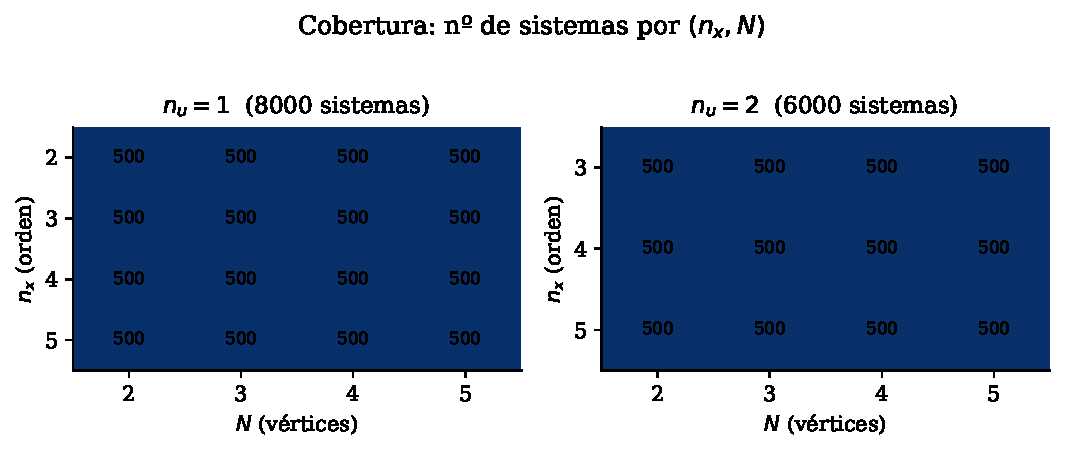
\includegraphics[width=\linewidth]{fig1_cobertura.pdf}
  \caption{Cobertura factorial: número de sistemas por $(n_x,N)$, separado por
  número de actuadores $n_u$. El soporte está completamente balanceado a $500$
  sistemas por celda.}
  \label{fig:cobertura}
\end{figure}

% --------------------------------------------------------------------
\subsection{La planta sin control (lazo abierto)}
\label{sec:db-ol}
% --------------------------------------------------------------------

``Lazo abierto'' se refiere al sistema \emph{sin} controlador. Las plantas de la
base son \emph{difíciles}: el $\mathbf{98.8\%}$ es inestable en lazo abierto
(al menos un vértice tiene un autovalor con parte real positiva), y sólo el
$1.2\%$ sería estable por sí solo. La abscisa espectral del peor vértice
(la rapidez del modo más inestable, ver Sec.~\ref{sec:db-conceptos}) tiene
mediana $30.9$ y llega hasta $\sim\!832$ (Fig.~\ref{fig:estabilidad}). En otras
palabras, la base no contiene casos triviales: el controlador debe
\emph{crear} la estabilidad, no sólo conservarla.

\begin{figure}[t]
  \centering
  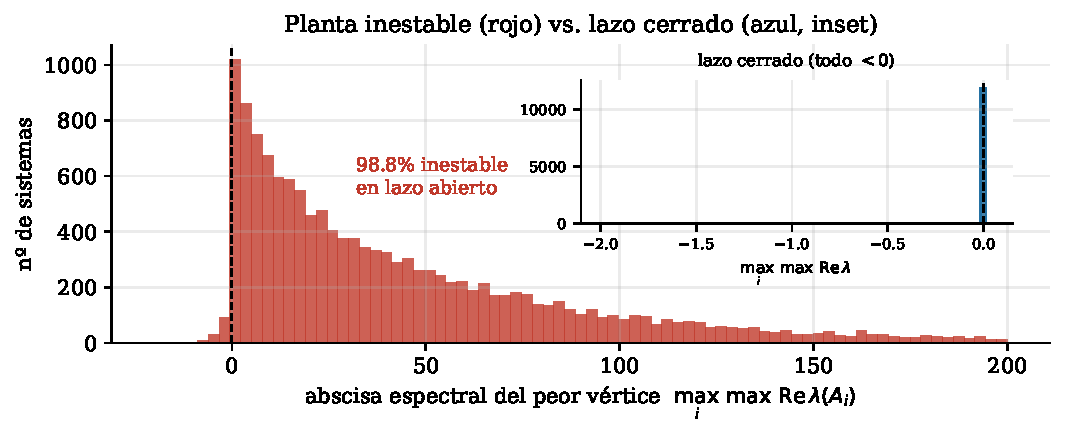
\includegraphics[width=\linewidth]{fig2_estabilidad.pdf}
  \caption{Abscisa espectral del peor vértice. Sin control la planta es
  inestable (rojo, parte real $>0$) en el $98.8\%$ de los casos; con la ganancia
  $K$ el lazo cerrado es estable en el $100\%$ (inset azul, todos $<0$).}
  \label{fig:estabilidad}
\end{figure}

En cuanto al ``tamaño'' de la dinámica (Fig.~\ref{fig:normas}), los descriptores
tienen un rango muy amplio: $\max_i\lVert A_i\rVert_2$ va de $12$ a $1012$
(mediana $131$) y crece de forma marcada con el orden $n_x$, mientras que
$\max_i\lVert B_i\rVert_2$ se mantiene acotado en $[0.74,\,16.8]$. Esta
disparidad de escalas —tres órdenes de magnitud en $\lVert A\rVert$— es
justamente la que obliga a \emph{normalizar} los datos antes de entrenar: cada
politopo se reescala dividiéndolo por su entrada de mayor magnitud,
$\gamma=\max(\max|A|,\max|B|)$, de modo que todas las cifras queden en
$[-1,1]$ y los sistemas sean comparables entre sí (esta reescala no cambia el
signo de los autovalores —y por tanto no afecta la estabilidad— aunque sí divide
la tasa de decaimiento por $\gamma$).

\begin{figure}[t]
  \centering
  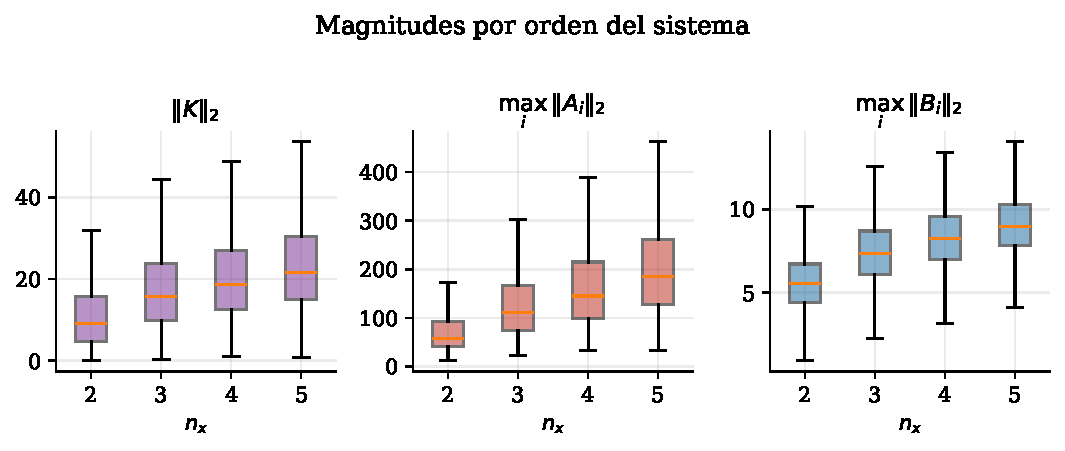
\includegraphics[width=\linewidth]{fig5_normas.pdf}
  \caption{Distribución del esfuerzo de control $\lVert K\rVert_2$ y de los
  tamaños $\max_i\lVert A_i\rVert_2$ y $\max_i\lVert B_i\rVert_2$, según el orden
  $n_x$. Ambos crecen con el orden del sistema.}
  \label{fig:normas}
\end{figure}

\paragraph{¿Se puede controlar? Controlabilidad y condicionamiento.}
Un requisito previo para que exista una ganancia estabilizante es que el sistema
sea \emph{controlable}: que desde la entrada se pueda influir en todas las
direcciones del estado. Esto se cumple en el $100\%$ de los vértices de todos
los sistemas. El número de condición de las matrices es benigno en general
($\kappa(A_i)$ con mediana $53$), con una cola pesada: un $0.39\%$ de los
sistemas supera $\kappa>10^4$, con casos extremos de hasta $5.7\times10^5$
(Fig.~\ref{fig:cond}); estos son los sistemas numéricamente delicados durante el
entrenamiento.

\begin{figure}[t]
  \centering
  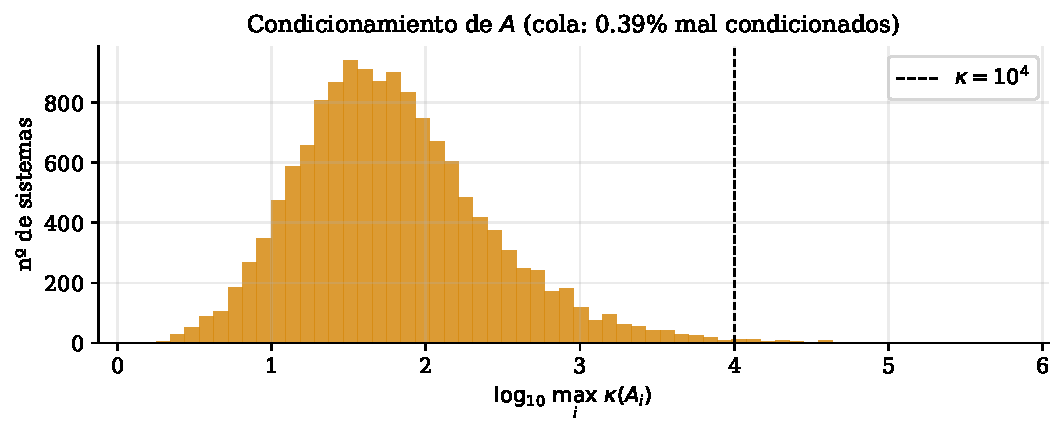
\includegraphics[width=0.82\linewidth]{fig7_condicionamiento.pdf}
  \caption{Número de condición $\max_i\kappa(A_i)$ (escala $\log_{10}$). La gran
  mayoría está bien condicionada; una cola del $0.39\%$ supera $\kappa=10^4$.}
  \label{fig:cond}
\end{figure}

% --------------------------------------------------------------------
\subsection{Tamaño de la incertidumbre (geometría del politopo)}
% --------------------------------------------------------------------

¿Qué tan ``grande'' es la incertidumbre de cada sistema? Lo medimos con la
dispersión de los vértices respecto a su promedio,
$\max_i\lVert A_i-\bar A\rVert_2$: si los vértices son muy parecidos entre sí, el
politopo es pequeño (poca incertidumbre); si son muy distintos, es grande. Su
mediana es $97.5$ y crece de forma sistemática con el número de vértices $N$
(Fig.~\ref{fig:dispersion}): más vértices implican politopos más amplios y, por
tanto, una incertidumbre más severa que la \emph{misma} ganancia $K$ debe cubrir
a la vez. Esto convierte a $N$ en un eje natural de dificultad y motiva evaluar
el modelo \emph{separado por $N$}.

\begin{figure}[t]
  \centering
  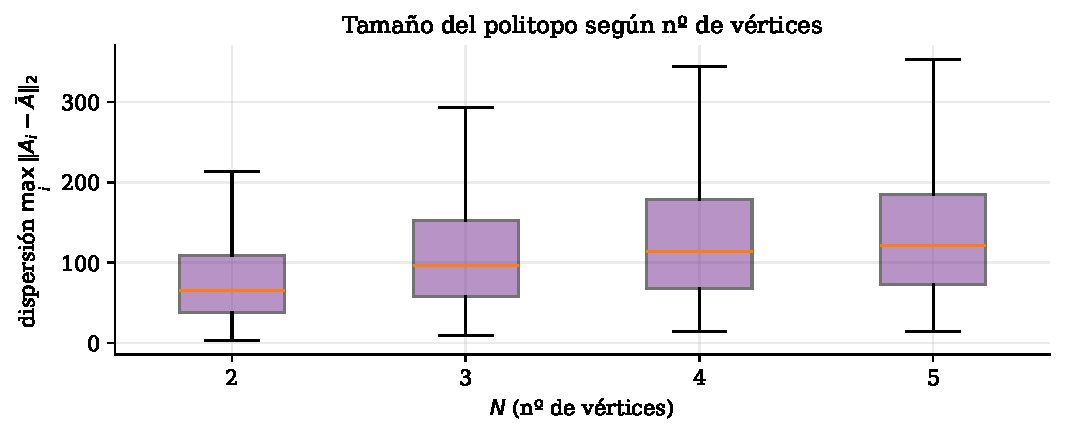
\includegraphics[width=0.82\linewidth]{fig6_dispersion.pdf}
  \caption{Tamaño del politopo $\max_i\lVert A_i-\bar A\rVert_2$ frente al número
  de vértices $N$. La incertidumbre crece con $N$.}
  \label{fig:dispersion}
\end{figure}

% --------------------------------------------------------------------
\subsection{El controlador y el sistema en lazo cerrado}
\label{sec:db-control}
% --------------------------------------------------------------------

``Lazo cerrado'' es el sistema \emph{con} el controlador conectado, gobernado por
$A_i+B_iK$. Verificamos numéricamente la etiqueta de la base recomputando los
autovalores de todos los vértices con su ganancia. El resultado es categórico:
\textbf{el $100\%$ de los $14\,000$ sistemas queda estable} (todos los
autovalores de todos los vértices con parte real negativa). No hay sistemas mal
etiquetados ni ganancias inconsistentes.

\paragraph{Estabilización ``al borde''.}
Lo más informativo es \emph{cómo} se estabiliza. La tasa de decaimiento lograda
$\alpha$ (Sec.~\ref{sec:db-conceptos}) —cuánto margen de estabilidad consigue el
controlador— se concentra masivamente junto a cero: su mediana es
$\alpha\approx 6.3\times10^{-4}$ y el $\mathbf{84.9\%}$ de los sistemas queda
\emph{casi marginal} ($\alpha<10^{-2}$), con sólo una minoría que alcanza
márgenes amplios ($\alpha_{95}=1.51$, máximo $10.6$). La distribución es
claramente \emph{bimodal} (Fig.~\ref{fig:decay}). Es decir, la ganancia de
referencia \emph{apenas} estabiliza: deja el modo dominante prácticamente sobre
la frontera de la inestabilidad.

\begin{figure}[t]
  \centering
  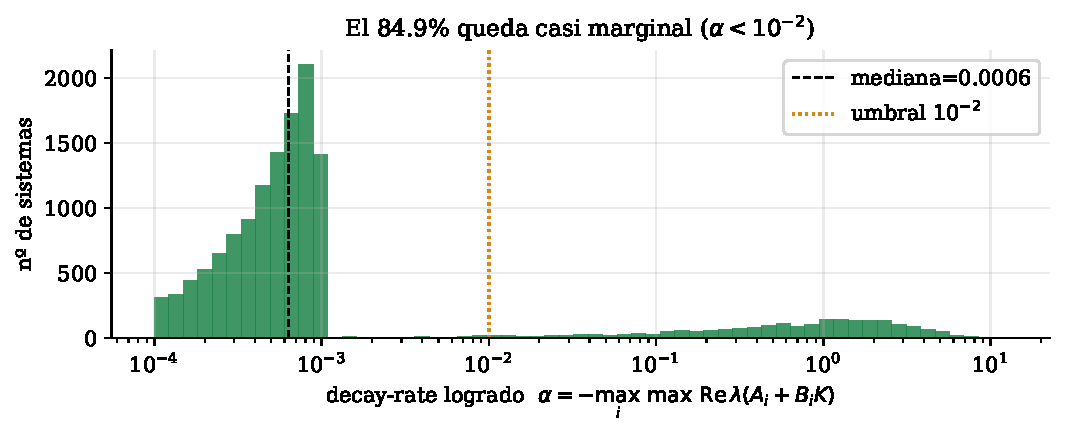
\includegraphics[width=\linewidth]{fig3_decay.pdf}
  \caption{Tasa de decaimiento lograda $\alpha$ (escala logarítmica). El
  $84.9\%$ de los sistemas queda casi marginal ($\alpha<10^{-2}$); una minoría
  exhibe márgenes grandes. La distribución es bimodal.}
  \label{fig:decay}
\end{figure}

Este comportamiento sugiere que las ganancias se construyeron buscando
\emph{cualquier} solución válida (factibilidad), no la más rápida. Lo respalda
un detalle: aunque el modo \emph{dominante} se aparca en la frontera, el resto de
los modos se empujan muy hacia la zona estable —la mediana de la parte real
sobre \emph{todos} los autovalores de lazo cerrado es $-21.4$. Visualmente, el
controlador ``refleja'' el espectro de la planta desde el semiplano inestable
(derecho) al estable (izquierdo), dejando un único modo lento que fija $\alpha$
(Fig.~\ref{fig:plano}).

\begin{figure}[t]
  \centering
  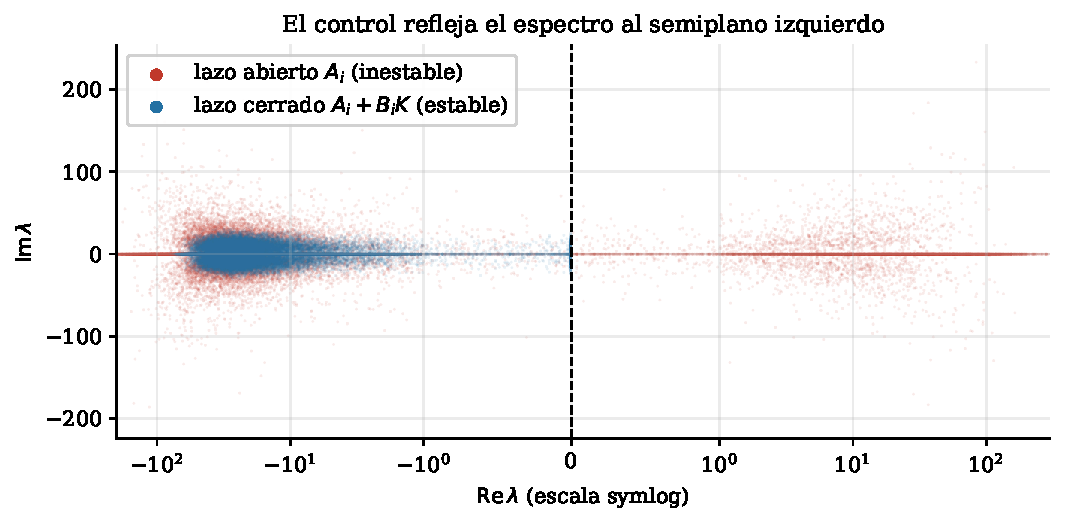
\includegraphics[width=\linewidth]{fig4_plano_complejo.pdf}
  \caption{Autovalores de los vértices en el plano complejo (eje horizontal en
  escala symlog). Sin control (rojo) la planta tiene autovalores en el semiplano
  derecho (inestables); con control (azul) todos pasan al semiplano izquierdo
  (estables), con el modo dominante pegado al eje.}
  \label{fig:plano}
\end{figure}

\paragraph{Esfuerzo de control.}
Lo ``caro'' que resulta controlar cada sistema se mide con $\lVert K\rVert_2$
(mediana $17.4$, máximo $98.1$). No es arbitrario: crece junto con el tamaño de
la planta ($\rho_{\text{Spearman}}=0.90$ frente a $\lVert A\rVert$), el tamaño
del politopo ($0.85$ frente a la dispersión) y la inestabilidad de lazo abierto
($0.63$); plantas más grandes e inestables exigen controladores más fuertes
(Fig.~\ref{fig:corr}). En cambio, la tasa de decaimiento $\alpha$ es
\emph{estadísticamente independiente} de todos los descriptores ($|\rho|\le0.04$
en todos los casos): el margen marginal no se debe a que el problema sea difícil,
sino a la forma en que se construyó la ganancia.

\begin{figure}[t]
  \centering
  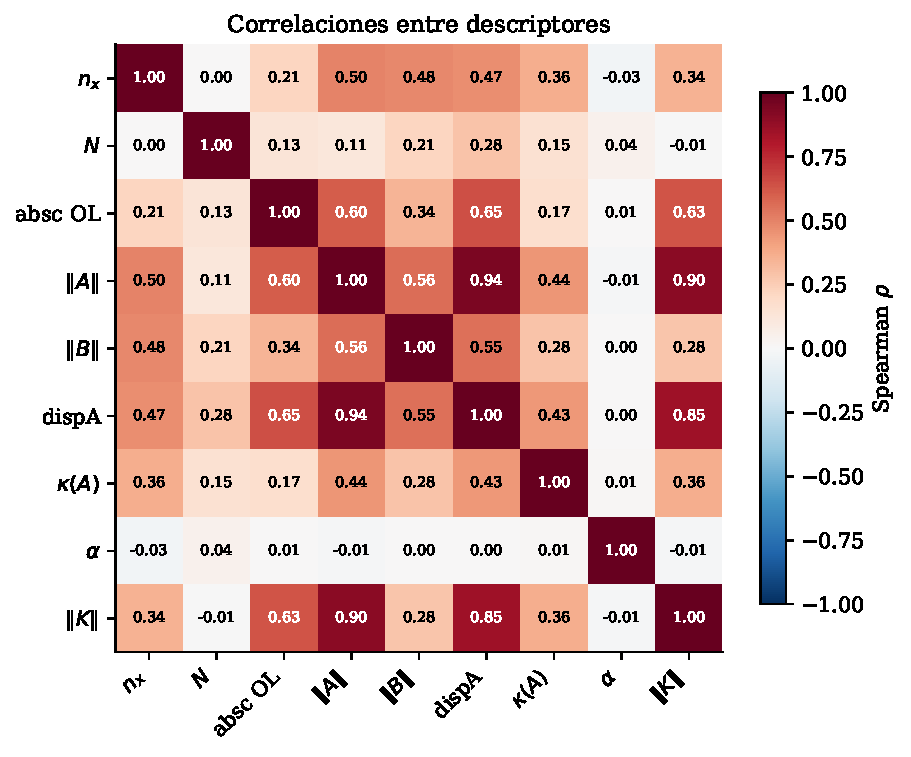
\includegraphics[width=0.78\linewidth]{fig8_correlaciones.pdf}
  \caption{Correlaciones de rango (Spearman) entre indicadores. El esfuerzo
  $\lVert K\rVert$ sigue al tamaño de la planta y del politopo; la tasa de
  decaimiento $\alpha$ no correlaciona con ningún indicador.}
  \label{fig:corr}
\end{figure}

% --------------------------------------------------------------------
\subsection{Calidad de los datos}
% --------------------------------------------------------------------

\begin{itemize}
  \item \textbf{Completitud:} sin valores faltantes en el soporte; las $28$
        celdas válidas están pobladas a $500/500$.
  \item \textbf{Validez de la etiqueta:} $100\%$ de los sistemas verificados como
        efectivamente estabilizados por su $K$ (todos los vértices estables).
  \item \textbf{Controlabilidad:} $100\%$ de los vértices controlables.
  \item \textbf{Duplicados:} no se detectaron sistemas repetidos.
  \item \textbf{Valores atípicos:} acotados y plausibles; la única cola de
        cuidado es el condicionamiento numérico ($0.39\%$ con $\kappa>10^4$),
        relevante para la estabilidad del cálculo más que para la validez del dato.
\end{itemize}

\begin{table}[t]
  \centering
  \caption{Resumen de indicadores sobre los $14\,000$ sistemas (datos crudos,
  sin normalizar).}
  \label{tab:resumen}
  \begin{tabular}{lrrr}
    \toprule
    Indicador & Mín. & Mediana & Máx. \\
    \midrule
    Abscisa espectral peor vértice (sin control) & $-17.9$ & $30.9$ & $832$ \\
    Tasa de decaimiento lograda $\alpha$         & $1.0\times10^{-4}$ & $6.3\times10^{-4}$ & $10.6$ \\
    $\max_i\lVert A_i\rVert_2$ (tamaño de la dinámica) & $12.2$ & $131$ & $1012$ \\
    $\max_i\lVert B_i\rVert_2$ (autoridad del control) & $0.74$ & $7.90$ & $16.8$ \\
    Dispersión del politopo (incertidumbre)      & $3.12$ & $97.5$ & $850$ \\
    Condición $\max_i\kappa(A_i)$                 & $1.44$ & $52.8$ & $5.7\times10^{5}$ \\
    Esfuerzo de control $\lVert K\rVert_2$        & $0.077$ & $17.4$ & $98.1$ \\
    \bottomrule
  \end{tabular}
\end{table}

% --------------------------------------------------------------------
\subsection{Implicaciones para el aprendizaje}
% --------------------------------------------------------------------

El análisis orienta varias decisiones de modelado:
%
\begin{enumerate}
  \item \textbf{Normalización imprescindible.} El rango de tamaños de $\lVert
        A\rVert$ (tres órdenes de magnitud) hace inviable alimentar las matrices
        crudas a la red; la reescala por $\gamma$ es necesaria para que el
        aprendizaje esté bien condicionado.
  \item \textbf{Invarianzas a aprovechar.} Un sistema es un \emph{conjunto} de
        vértices $\{(A_i,B_i)\}$ cuyo orden no importa y cuya cantidad $N$ varía,
        pero el certificado $K$ es común; esto motiva un codificador invariante
        al orden y a la cantidad de vértices (y, análogamente, al número de
        actuadores $n_u$).
  \item \textbf{Evaluar separado por $N$.} Como la incertidumbre crece con el
        número de vértices, conviene reportar el desempeño desglosado por $N$.
  \item \textbf{Sobre la señal de entrenamiento.} La ganancia de referencia es
        casi marginal y su $\alpha$ no aporta información sobre el sistema; esto
        respalda usar un objetivo \emph{auto-supervisado} —estabilizar con un
        margen $\alpha$ prescrito— en lugar de copiar directamente la $K$
        almacenada.
\end{enumerate}

%  Requiere: graphicx, booktabs, amsmath, amssymb
%  \graphicspath{{figuras/}}  % o ajusta la ruta a tus figuras
% =====================================================================

\section{Caracterización de la base de datos}
\label{sec:analisis-db}


% --------------------------------------------------------------------
\subsection{Cómo se mide un sistema y su estabilidad}
\label{sec:db-conceptos}
% --------------------------------------------------------------------



\paragraph{Abscisa espectral.}
La abscisa espectral es el mayor de las partes reales,
$\max\operatorname{Re}\lambda(A)$. Es el modo que crece más rápido (o decae más
lento) y, por sí solo, decide la estabilidad: si la abscisa es negativa, todos
los modos decaen; si es positiva, al menos uno explota. Un valor de, por
ejemplo, $832$ significa que el modo dominante crece como $e^{832\,t}$: una
inestabilidad extremadamente violenta. Lo usamos como \emph{medida relativa de
qué tan inestable} es una planta (no tiene unidades físicas porque los sistemas
son sintéticos).

\paragraph{Los dos ``máximos''.}
En las fórmulas aparecen \emph{dos} máximos anidados, y conviene separarlos:
%
\begin{equation*}
  \underbrace{\max_{i=1,\dots,N}}_{\text{(2) peor \emph{vértice}}}
  \ \underbrace{\max\,\operatorname{Re}\,\lambda(A_i)}_{\text{(1) peor \emph{modo} de ese vértice}}.
\end{equation*}
%
El máximo interno (1) recorre los autovalores de \emph{un} vértice y se queda
con su modo dominante (la abscisa espectral de $A_i$). El máximo externo (2)
recorre los $N$ vértices del politopo y se queda con el más desfavorable. La
combinación es la lectura de \emph{peor caso}: ``de toda la familia de sistemas
posibles, ¿qué tan mal se comporta el peor de ellos?''.

\paragraph{Norma de una matriz: su ``tamaño''.}
La norma espectral $\lVert A\rVert_2$ mide cuánto puede \emph{amplificar} esa
matriz a un vector (formalmente, su mayor valor singular). Es una medida del
``tamaño'' o la fuerza de la dinámica: una $\lVert A\rVert_2$ grande indica
acoplamientos internos intensos. Reportamos $\max_i\lVert A_i\rVert_2$, el
tamaño del vértice más grande del politopo.

\paragraph{Tasa de decaimiento $\alpha$: el margen de seguridad.}
Una vez cerrado el lazo con el controlador, la matriz que gobierna la dinámica
pasa a ser $A_i+B_iK$. Su abscisa espectral, cambiada de signo, es la
\textbf{tasa de decaimiento}
$\alpha=-\max_i\max\operatorname{Re}\lambda(A_i+B_iK)$. Mide \emph{qué tan
rápido} se extingue la peor respuesta: $\alpha>0$ garantiza estabilidad, y
cuanto mayor sea $\alpha$, más rápido y con más margen vuelve el sistema al
equilibrio. Un $\alpha\approx0$ significa ``estable, pero al borde'': el sistema
apenas se sostiene sobre la frontera de la inestabilidad.

\paragraph{Otros indicadores.}
La \emph{dispersión del politopo} $\max_i\lVert A_i-\bar A\rVert_2$ (con $\bar A$
el promedio de los vértices) mide qué tan distintos son los vértices entre sí,
es decir, cuánta incertidumbre hay. El \emph{número de condición} $\kappa(A_i)$
mide la sensibilidad numérica de la matriz (valores altos anticipan problemas de
precisión). El \emph{esfuerzo de control} $\lVert K\rVert_2$ mide qué tan
``agresivo'' es el controlador.

\begin{table}[t]
  \centering
  \caption{Glosario de indicadores usados en el análisis.}
  \label{tab:glosario}
  \small
  \begin{tabular}{p{3.0cm}p{3.4cm}p{6.6cm}}
    \toprule
    Indicador & En palabras simples & Un valor alto significa\dots \\
    \midrule
    Abscisa espectral (lazo abierto)\newline $\max_i\max\operatorname{Re}\lambda(A_i)$
      & Rapidez del modo más inestable del peor vértice
      & Planta muy inestable: sin control, se dispara muy rápido. \\
    Tasa de decaimiento\newline $\alpha=-\max_i\max\operatorname{Re}\lambda(A_i+B_iK)$
      & Qué tan rápido se calma el sistema ya controlado
      & Más margen de estabilidad; $\alpha\approx0$ = estable al borde. \\
    Norma $\max_i\lVert A_i\rVert_2$
      & ``Tamaño''/fuerza de la dinámica propia
      & Acoplamientos internos intensos. \\
    Norma $\max_i\lVert B_i\rVert_2$
      & Cuánto influye el control en el estado
      & Actuadores con mucha autoridad. \\
    Dispersión del politopo\newline $\max_i\lVert A_i-\bar A\rVert_2$
      & Qué tan distintos son los vértices
      & Más incertidumbre que cubrir con una sola $K$. \\
    Condición $\kappa(A_i)$
      & Sensibilidad numérica de la matriz
      & Riesgo de imprecisión numérica. \\
    Esfuerzo $\lVert K\rVert_2$
      & Qué tan ``fuerte'' es el controlador
      & Acción de control más agresiva. \\
    \bottomrule
  \end{tabular}
\end{table}





% --------------------------------------------------------------------
\subsection{Propósito y estructura}
% --------------------------------------------------------------------

El conjunto de datos utilizado reúne sistemas lineales
\emph{politópicos} de tiempo continuo junto con una ley de realimentación de
estado estática (\emph{static state feedback}) que los estabiliza de forma
robusta. Cada muestra es una terna $(\mathcal{A},\mathcal{B},K)$ donde el sistema
incierto se describe como la envolvente convexa de $N$ vértices,
%
\begin{equation}
  \dot{x}(t) = A(\theta)\,x(t) + B(\theta)\,u(t),
  \qquad
  \bigl(A(\theta),B(\theta)\bigr)=\sum_{i=1}^{N}\theta_i\,(A_i,B_i),
  \quad \theta_i\ge 0,\ \textstyle\sum_i\theta_i=1,
  \label{eq:politopo}
\end{equation}
%
con $A_i\in\mathbb{R}^{n_x\times n_x}$, $B_i\in\mathbb{R}^{n_x\times n_u}$, y
$K\in\mathbb{R}^{n_u\times n_x}$ la ganancia común a todo el politopo, de modo
que $u=Kx$. La etiqueta \texttt{RS} indica que el sistema es robustamente (cuadráticamente)
estabilizable.\footnote{\textbf{Procedencia (por confirmar con el autor de la base):}
la evidencia empírica (Sec.~\ref{sec:db-control}) es consistente con que cada $K$
se obtuvo resolviendo una LMI de estabilizabilidad cuadrática con un certificado
común $(Q,Y)$ y $K=YQ^{-1}$, sin maximizar la tasa de decaimiento. Falta confirmar
el procedimiento exacto de muestreo de los vértices $(A_i,B_i)$.}

El archivo organiza las muestras en un arreglo de celdas de cuatro índices,
$\texttt{BASE}[\,n_x,\,n_u,\,N,\,\text{caso}\,]$, de forma nominal
$5\times 2\times 5\times 500$. Cada celda poblada contiene los campos
\texttt{A} (celda de $N$ matrices $A_i$), \texttt{B} (celda de $N$ matrices $B_i$)
y \texttt{K}. La malla está poblada parcialmente: el orden mínimo depende del
número de actuadores ($n_u{=}1\Rightarrow n_x\in\{2,\dots,5\}$;
$n_u{=}2\Rightarrow n_x\in\{3,4,5\}$) y siempre $N\ge 2$, de modo que de las
$25\,000$ posiciones nominales sólo $28$ celdas están ocupadas, con
exactamente $500$ casos cada una: en total $\mathbf{14\,000}$ sistemas
($8\,000$ con $n_u{=}1$ y $6\,000$ con $n_u{=}2$).

\begin{table}[t]
  \centering
  \caption{Esquema de la base de datos. Cada sistema es un politopo de $N$
  vértices con una ganancia robusta $K$.}
  \label{tab:esquema}
  \begin{tabular}{llll}
    \toprule
    Campo & Símbolo & Forma & Descripción \\
    \midrule
    \texttt{A} & $\{A_i\}_{i=1}^N$ & $N\times(n_x\!\times\! n_x)$ & Matrices de estado de los vértices \\
    \texttt{B} & $\{B_i\}_{i=1}^N$ & $N\times(n_x\!\times\! n_u)$ & Matrices de entrada de los vértices \\
    \texttt{K} & $K$               & $n_u\times n_x$             & Ganancia de realimentación común \\
    \midrule
    \multicolumn{4}{l}{$n_x\in\{2,3,4,5\}$\quad $n_u\in\{1,2\}$\quad $N\in\{2,3,4,5\}$\quad $500$ casos/celda} \\
    \bottomrule
  \end{tabular}
\end{table}

% --------------------------------------------------------------------
\subsection{Cobertura y diseño experimental}
% --------------------------------------------------------------------

La base sigue un \emph{diseño factorial completo y perfectamente balanceado}
sobre los factores $(n_x, n_u, N)$ admisibles
(Fig.~\ref{fig:cobertura}): las $28$ combinaciones válidas aparecen con la
misma cardinalidad ($500$), sin celdas faltantes ni sobre-representadas dentro
del soporte. Este balance es deseable para el aprendizaje: evita que el modelo
privilegie una topología por mero desbalance de frecuencia y permite reportar
métricas estratificadas por $N$ y por $n_x$ sin ponderaciones correctoras.

\begin{figure}[t]
  \centering
  
\includegraphics[width=\linewidth]{2da Versión/Capitulos/figuras/fig1_cobertura.pdf}
  \caption{Cobertura factorial: número de sistemas por $(n_x,N)$, separado por
  número de actuadores $n_u$. El soporte está completamente balanceado a
  $500$ sistemas por celda.}
  \label{fig:cobertura}
\end{figure}

% --------------------------------------------------------------------
\subsection{La planta en lazo abierto}
\label{sec:db-ol}
% --------------------------------------------------------------------

Las plantas son \emph{difíciles}: el $\mathbf{98.8\%}$ de los sistemas es
inestable en lazo abierto (al menos un vértice con autovalores en el semiplano
derecho), y sólo un $1.2\%$ es estable sin control. La abscisa espectral del
peor vértice, $\max_i\max\operatorname{Re}\lambda(A_i)$, tiene mediana $30.9$
y alcanza valores de hasta $\sim\!832$ (Fig.~\ref{fig:estabilidad}). Es decir,
la base no contiene plantas triviales: el controlador debe \emph{crear} la
estabilidad, no solo preservarla.

\begin{figure}[t]
  \centering
  
\includegraphics[width=\linewidth]{2da Versión/Capitulos/figuras/fig2_estabilidad.pdf}
  \caption{Abscisa espectral del peor vértice. La planta es inestable
  (rojo, $\operatorname{Re}\lambda>0$) en el $98.8\%$ de los casos; bajo la ganancia
  $K$ el lazo cerrado es estable en el $100\%$ (inset azul, todos $<0$).}
  \label{fig:estabilidad}
\end{figure}

En cuanto a las magnitudes (Fig.~\ref{fig:normas}), los descriptores presentan
un rango dinámico amplio: $\max_i\lVert A_i\rVert_2$ va de $12$ a $1012$
(mediana $131$) y crece de forma marcada con el orden $n_x$, mientras que
$\max_i\lVert B_i\rVert_2$ se mantiene acotado en $[0.74,\,16.8]$. Esta
disparidad de escalas —tres órdenes de magnitud en $\lVert A\rVert$— es
precisamente la que justifica la \emph{normalización física} aplicada en la
ingesta: cada politopo se reescala por $\gamma=\max(\max|A|,\max|B|)$ antes de
entrar a la red, llevando todas las entradas a $[-1,1]$ y homogeneizando las
escalas entre sistemas (la normalización preserva el signo de los autovalores,
luego no altera la propiedad de estabilizabilidad, aunque escala la tasa de
decaimiento por $1/\gamma$).

\begin{figure}[t]
  \centering
  
\includegraphics[width=\linewidth]{2da Versión/Capitulos/figuras/fig5_normas.pdf}
  \caption{Distribución de $\lVert K\rVert_2$, $\max_i\lVert A_i\rVert_2$ y
  $\max_i\lVert B_i\rVert_2$ por orden $n_x$ (cajas sin \emph{outliers}). El
  esfuerzo de control y la norma de la planta crecen con el orden.}
  \label{fig:normas}
\end{figure}

\paragraph{Controlabilidad y condicionamiento.}
\textcolor{blue}{Revisar esa condición, estaría interesante agregarla al marco teórico. }Todos los vértices de todos los sistemas son controlables (rango pleno de la
matriz de controlabilidad $[\,B_i\ A_iB_i\ \cdots\ A_i^{n_x-1}B_i\,]$ en el
$100\%$ de los casos), condición necesaria para la existencia de una ganancia
estabilizante. El condicionamiento de las matrices de estado es benigno en
general ($\kappa(A_i)$ con mediana $53$), con una cola pesada: un $0.39\%$ de
los sistemas presenta $\kappa>10^4$ y casos extremos de hasta $5.7\times10^5$
(Fig.~\ref{fig:cond}), un detalle relevante para la estabilidad numérica del
solver durante el entrenamiento.

\begin{figure}[t]
  \centering
  
\includegraphics[width=0.82\linewidth]{2da Versión/Capitulos/figuras/fig7_condicionamiento.pdf}
  \caption{Condicionamiento $\max_i\kappa(A_i)$ (escala $\log_{10}$). La gran
  mayoría está bien condicionada; una cola del $0.39\%$ supera $\kappa=10^4$.}
  \label{fig:cond}
\end{figure}

% --------------------------------------------------------------------
\subsection{Geometría del politopo}
% --------------------------------------------------------------------

La ``extensión'' de la incertidumbre se mide con la dispersión de los vértices
respecto a su centroide, $\operatorname{dispA}=\max_i\lVert A_i-\bar A\rVert_2$.
Su mediana es $97.5$ y crece de manera sistemática con el número de vértices
$N$ (Fig.~\ref{fig:dispersion}): más vértices implican politopos más grandes y,
por tanto, una incertidumbre más severa que el mismo certificado $K$ debe
cubrir simultáneamente. Esto vuelve a $N$ un eje de dificultad natural y
motiva evaluar el modelo \emph{estratificado por $N$}.

\begin{figure}[t]
  \centering
  
\includegraphics[width=0.82\linewidth]{2da Versión/Capitulos/figuras/fig6_dispersion.pdf}
  \caption{Tamaño del politopo $\max_i\lVert A_i-\bar A\rVert_2$ frente al
  número de vértices $N$. La incertidumbre crece con $N$.}
  \label{fig:dispersion}
\end{figure}

% --------------------------------------------------------------------
\subsection{La ley de control y el lazo cerrado}
\label{sec:db-control}
% --------------------------------------------------------------------

Verificamos numéricamente la etiqueta de la base recomputando, para cada
sistema, los autovalores de lazo cerrado de todos los vértices
$A_i+B_iK$. El resultado es categórico: \textbf{el $100\%$ de los $14\,000$
sistemas queda con todos sus vértices en el semiplano izquierdo}, es decir,
la ganancia almacenada estabiliza efectivamente cada politopo. No se hallaron
sistemas mal etiquetados ni ganancias inconsistentes.

\paragraph{Estabilización al borde.}
El \emph{cómo} se estabiliza es el hallazgo más informativo. La tasa de
decaimiento efectivamente lograda,
$\alpha=-\max_i\max\operatorname{Re}\lambda(A_i+B_iK)$, se concentra
masivamente junto a cero: la mediana es $\alpha\approx 6.3\times10^{-4}$ y el
$\mathbf{84.9\%}$ de los sistemas queda \emph{casi marginal}
($\alpha<10^{-2}$), con sólo una cola minoritaria que alcanza márgenes
apreciables ($\alpha_{95}=1.51$, máximo $10.6$). La distribución es claramente
bimodal (Fig.~\ref{fig:decay}). En otras palabras, la ganancia de referencia
\emph{apenas} estabiliza: coloca el polo dominante prácticamente sobre el eje
imaginario.

\begin{figure}[t]
  \centering
  
\includegraphics[width=\linewidth]{2da Versión/Capitulos/figuras/fig3_decay.pdf}
  \caption{Tasa de decaimiento lograda $\alpha$ (escala log). El $84.9\%$ de
  los sistemas queda casi marginal ($\alpha<10^{-2}$); una minoría exhibe
  márgenes grandes. La distribución es bimodal.}
  \label{fig:decay}
\end{figure}

Este comportamiento es coherente con una construcción de $K$ orientada a la
\emph{factibilidad} de la LMI (encontrar cualquier certificado válido), no a
la optimización del decaimiento. Lo respalda el hecho de que, aunque el polo
\emph{dominante} se aparca en el eje, el resto del espectro se empuja muy hacia
la izquierda: la mediana de la parte real sobre \emph{todos} los autovalores de
lazo cerrado es $-21.4$. El controlador, en efecto, ``refleja'' el espectro de
la planta del semiplano derecho al izquierdo (Fig.~\ref{fig:plano}), dejando un
único modo lento que fija $\alpha$.

\begin{figure}[t]
  \centering
  
\includegraphics[width=\linewidth]{2da Versión/Capitulos/figuras/fig4_plano_complejo.pdf}
  \caption{Autovalores de los vértices en el plano complejo (escala symlog en
  el eje real). La planta en lazo abierto (rojo) se extiende al semiplano
  derecho; el lazo cerrado (azul) queda íntegramente a la izquierda, con el
  polo dominante junto al eje.}
  \label{fig:plano}
\end{figure}

\paragraph{Esfuerzo de control.}
El esfuerzo $\lVert K\rVert_2$ tiene mediana $17.4$ y máximo $98.1$. No es
gratuito: correlaciona fuertemente con la norma de la planta
($\rho_{\text{Spearman}}=0.90$ con $\lVert A\rVert$), con el tamaño del
politopo ($0.85$ con $\operatorname{dispA}$) y con la inestabilidad de lazo
abierto ($0.63$); plantas más grandes e inestables exigen ganancias mayores
(Fig.~\ref{fig:corr}). En contraste, $\alpha$ es \emph{estadísticamente
independiente} de todos los descriptores del sistema ($|\rho|\le 0.04$ en todos
los casos), lo que confirma que el margen marginal no responde a la dificultad
del problema sino a la propia construcción de la ganancia.

\begin{figure}[t]
  \centering
  
\includegraphics[width=0.78\linewidth]{2da Versión/Capitulos/figuras/fig8_correlaciones.pdf}
  \caption{Correlaciones de Spearman entre descriptores. $\lVert K\rVert$ sigue
  a $\lVert A\rVert$ y a la dispersión del politopo; la tasa de decaimiento
  $\alpha$ no correlaciona con ningún descriptor.}
  \label{fig:corr}
\end{figure}

% --------------------------------------------------------------------
\subsection{Calidad de los datos}
% --------------------------------------------------------------------

\begin{itemize}
  \item \textbf{Completitud:} sin valores faltantes en el soporte; las $28$
        celdas válidas están pobladas a $500/500$.
  \item \textbf{Validez de etiqueta:} $100\%$ de los sistemas verificados como
        robustamente estabilizados por su $K$ (todos los vértices Hurwitz).
  \item \textbf{Controlabilidad:} $100\%$ de los vértices controlables.
  \item \textbf{Duplicados:} no se detectaron sistemas repetidos.
  \item \textbf{Valores atípicos:} acotados y plausibles; la única cola de
        cuidado es el condicionamiento ($0.39\%$ con $\kappa>10^4$), relevante
        para la estabilidad numérica más que para la validez del dato.
\end{itemize}

\begin{table}[t]
  \centering
  \caption{Resumen de descriptores sobre los $14\,000$ sistemas (datos crudos,
  sin normalizar).}
  \label{tab:resumen}
  \begin{tabular}{lrrr}
    \toprule
    Descriptor & Mín. & Mediana & Máx. \\
    \midrule
    Abscisa espectral peor vértice (lazo abierto) & $-17.9$ & $30.9$ & $832$ \\
    Tasa de decaimiento lograda $\alpha$           & $1.0\times10^{-4}$ & $6.3\times10^{-4}$ & $10.6$ \\
    $\max_i\lVert A_i\rVert_2$                      & $12.2$ & $131$ & $1012$ \\
    $\max_i\lVert B_i\rVert_2$                      & $0.74$ & $7.90$ & $16.8$ \\
    Dispersión del politopo $\operatorname{dispA}$ & $3.12$ & $97.5$ & $850$ \\
    Condicionamiento $\max_i\kappa(A_i)$           & $1.44$ & $52.8$ & $5.7\times10^{5}$ \\
    Esfuerzo de control $\lVert K\rVert_2$         & $0.077$ & $17.4$ & $98.1$ \\
    \bottomrule
  \end{tabular}
\end{table}

% --------------------------------------------------------------------
\subsection{Implicaciones para el aprendizaje}
% --------------------------------------------------------------------

El análisis sugiere varias decisiones de modelado:
%
\begin{enumerate}
  \item \textbf{Normalización imprescindible.} El rango dinámico de $\lVert
        A\rVert$ (tres décadas) hace inviable alimentar las matrices crudas; la
        reescala por $\gamma$ es necesaria para condicionar el aprendizaje.
  \item \textbf{Invarianzas a explotar.} El sistema es un \emph{conjunto} de
        vértices $\{(A_i,B_i)\}$ (invariante a permutación y a cardinalidad
        $N$) cuyo certificado $K$ es común; esto motiva un codificador
        invariante a $N$ y, análogamente, equivariante al número de actuadores
        $n_u$.
  \item \textbf{Estratificar por $N$.} Como la dificultad (tamaño del politopo)
        crece con $N$, conviene reportar el desempeño separado por número de
        vértices.
  \item \textbf{Sobre la señal de entrenamiento.} La ganancia de referencia es
        casi marginal y su $\alpha$ no informa sobre el sistema; esto avala
        usar un objetivo \emph{auto-supervisado} de factibilidad/volumen
        (estabilización con margen $\alpha$ prescrito) en lugar de regresar
        directamente la $K$ almacenada.
\end{enumerate}
